% =====================================================================
% CAPÍTULO 6 — Evaluación de modelos fundacionales
% Versión expandida según indicación de la profesora guía (cuerpo
% objetivo 85–100 páginas). El detalle exhaustivo (tablas completas,
% figuras de distribución y parches ejemplares) se encuentra en el
% Apéndice F.
% =====================================================================

\chapter{Evaluación de modelos fundacionales}
\label{cap:evaluacion_modelos}

El presente capítulo evalúa Phikon-v2, UNI2-h, Prov-GigaPath y Virchow2 en las cinco tareas definidas en el Capítulo~\ref{cap:seleccion_modelos}. El protocolo experimental se estructura en cuatro etapas: preprocesamiento de las \textit{Whole Slide Images} (WSI), extracción de representaciones visuales mediante los modelos fundacionales, entrenamiento de un clasificador sobre dichas representaciones y evaluación cuantitativa mediante métricas de utilidad, equidad y generalización. Cada etapa se describe con el nivel de detalle necesario para la reproducibilidad del estudio; los detalles de implementación y trazabilidad se documentan además en el material reproducible.

La evaluación se centra en tres dimensiones complementarias. La primera corresponde a la utilidad predictiva global, medida mediante \textit{balanced accuracy} (BA), macro-F1 y AUC, complementada con la sensibilidad (\textit{recall}) por clase para identificar qué clases se detectan de forma confiable. La segunda analiza la equidad del rendimiento entre subgrupos demográficos, particularmente sexo y grupo de edad, mediante brechas de desempeño. La tercera evalúa la generalización ante cambios de distribución, comparando el rendimiento \textit{in-distribution} (ID) y \textit{out-of-distribution} (OOD). Estas dimensiones se evalúan de forma conjunta para cada combinación de tarea, modelo y dataset, permitiendo una comparación sistemática del comportamiento de los modelos fundacionales en contextos clínicos diversos.

La interpretación integra BA, macro-F1, AUC, sensibilidad por clase e intervalos de confianza al 95\%. Las comparaciones entre tareas deben realizarse considerando sus diferencias en número de clases, prevalencias, tamaño muestral y disponibilidad de atributos demográficos; en particular, una \textit{balanced accuracy} similar puede tener implicancias distintas en una tarea binaria y en una tarea multiclase con categorías escasas.

\section{Protocolo experimental}
\label{sec:protocolo}

\subsection{Preprocesamiento y representaciones}
\label{sec:preprocesamiento_representaciones}
\label{sec:protocolo-inferencia}

Las WSI pueden alcanzar dimensiones de varios gigapíxeles y tamaños de archivo de entre 1 y 8 GB, lo que hace computacionalmente inviable procesarlas de manera directa y obliga a dividirlas en parches (\textit{patches}) de tamaño manejable para las arquitecturas basadas en \textit{Vision Transformers} (ViT). La extracción se realizó mediante un esquema de \textit{tiling} con ventana deslizante en tres etapas: apertura de la WSI y determinación del nivel de la pirámide de resolución más cercano a la magnificación objetivo, generación vectorizada de coordenadas de parches sobre la dimensión completa del \textit{slide}, y lectura de cada parche en su resolución correspondiente. Se generaron parches cuadrados no superpuestos de $224 \times 224$ px a una magnificación de $20\times$. El tamaño de parche corresponde a la entrada estándar de los \textit{encoders} ViT de los modelos fundacionales de patología digital publicados recientemente~\parencite{chen2024uni, filiot2024phikonv2}; utilizar el mismo tamaño que durante el preentrenamiento evita distorsiones por \textit{resize} adicional. La magnificación de $20\times$ se seleccionó por ser la predominante en los metadatos de adquisición de las cohortes, minimizando reescalados y la desalineación de dominio con la escala de entrenamiento de los \textit{encoders}.

Los parches extraídos se almacenaron en formato HDF5, organizados por WSI y agrupados dentro de un archivo por \textit{slide}. Este formato permite un acceso indexado eficiente a subconjuntos de parches sin descomprimir archivos individuales, soporta compresión interna (se utilizó el esquema \texttt{lzf}, que prioriza la velocidad de lectura/escritura sobre la tasa de compresión), permite escritura asíncrona mediante un hilo dedicado y evita la sobrecarga del sistema de archivos asociada a almacenar potencialmente millones de imágenes individuales por conjunto de datos. La Tabla~\ref{tab:patch_params} resume los parámetros de extracción, que se mantuvieron uniformes para todos los conjuntos de datos con el fin de reducir la variación atribuible al preprocesamiento.

\begin{table}[htbp]
    \centering
    \caption{Parámetros utilizados en la extracción de parches desde WSI.}
    \label{tab:patch_params}
    \begin{tabular}{p{4cm} p{3cm} p{7cm}}
        \toprule
        \textbf{Parámetro} & \textbf{Valor} & \textbf{Justificación} \\
        \midrule
        Tamaño de parche & $224 \times 224$ px & Tamaño de entrada estándar en modelos fundacionales de patología digital pre-entrenados  \\
        Magnificación & $20\times$ & Magnificación predominante en las cohortes evaluadas \\
        Desplazamiento & $224$ px & Sin solapamiento; prioriza eficiencia computacional y de almacenamiento sobre cobertura redundante \\
        Formato de salida & HDF5 & Acceso indexado eficiente, compresión interna (\texttt{lzf}), evita sobrecarga de sistema de archivos por millones de imágenes individuales \\
        \bottomrule
    \end{tabular}
\end{table}

Tras la extracción se aplicó un proceso de filtrado destinado a descartar parches sin tejido informativo o con artefactos de adquisición, que podrían afectar negativamente la extracción de representaciones. El filtrado opera sobre una miniatura de baja resolución de cada WSI (512$\times$512 o 1024$\times$1024 px, según configuración): sobre la miniatura convertida a escala de grises se calcula automáticamente un umbral mediante el método de Otsu, que maximiza la varianza entre clases (tejido/fondo) a partir del histograma de intensidades. A diferencia de un umbral fijo definido manualmente, el método de Otsu se adapta a la distribución de intensidades de cada imagen, lo que resulta más robusto frente a la variabilidad de tinción e iluminación entre cohortes; Prov-GigaPath aplica este método sobre imágenes reducidas para segmentar tejido y seleccionar los \textit{tiles} que serán procesados~\parencite{xu2024provgigapath}. Una vez generada la máscara binaria de tejido, cada parche candidato se proyecta sobre ella y se calcula la fracción de píxeles de tejido contenida en su área mediante una tabla de suma acumulada, lo que permite evaluar todos los parches de una WSI en una única operación vectorizada en lugar de iterar parche por parche. El umbral de tejido se fijó en 0,5 para todas las cohortes, en función de la proporción típica de tejido observada visualmente durante un proceso de calibración que incluyó un barrido de umbrales candidatos y la inspección visual de parches retenidos y descartados sobre muestras representativas de cada conjunto de datos.

El impacto del filtrado fue variable entre cohortes: la reducción del número de parches osciló entre 54,4\% en SurGen y 84,5\% en BCNB, reflejando diferencias en la calidad de las WSI y en las condiciones de adquisición de las imágenes (Tabla~\ref{tab:anexo_impacto_filtrado}, Apéndice~\ref{anexo:resultados_completos}).

Los parches retenidos se procesaron con Phikon-v2, UNI2-h, Prov-GigaPath y Virchow2 como extractores congelados, es decir, sin ajuste fino (\textit{fine-tuning}) de sus parámetros, con el objetivo de evaluar directamente la calidad de las representaciones aprendidas durante el preentrenamiento, siguiendo la práctica estándar de evaluación de modelos fundacionales mediante \textit{feature extraction}. Cada imagen se normalizó con las medias y desviaciones estándar asociadas al \textit{encoder} correspondiente, la extracción se ejecutó en modo de evaluación dentro de un contexto \texttt{torch.inference\_mode()} (evitando el cálculo y almacenamiento de gradientes) y los \textit{embeddings} se almacenaron junto con las coordenadas espaciales de sus parches, conservando la correspondencia entre cada representación y su ubicación original en la WSI. Cabe señalar que Prov-GigaPath fue preentrenado con parches de $256 \times 256$ px~\parencite{xu2024provgigapath}, mientras que en este estudio todos los modelos se evaluaron a $224 \times 224$ px; las representaciones de Prov-GigaPath se obtienen, por tanto, a una resolución menor que la de su preentrenamiento, una diferencia metodológica que debe considerarse al comparar su desempeño con el de los demás encoders.

La agregación desde el nivel de parche hasta el nivel de paciente se realizó en dos etapas de promedio aritmético: en primer lugar se promediaron los \textit{embeddings} de los parches de cada WSI y, en segundo lugar, los vectores de las WSI de un mismo paciente, de modo que cada paciente queda representado por un único vector de dimensión $D$ independientemente del número de parches y WSI disponibles. La verificación de integridad incluyó la confirmación de que la dimensión del \textit{embedding} coincide con la reportada por cada modelo en su documentación oficial, la detección de valores faltantes (\texttt{NaN}) o infinitos, y la validación de que cada paciente posee exactamente un \textit{embedding} final tras la etapa de agregación; los resultados se registraron en archivos de log para trazabilidad. Las dimensiones y entradas de los encoders se resumen en la Tabla~\ref{tab:embedding_models}.

\begin{table}[h]
\centering
\caption{Características de los modelos fundacionales utilizados para extracción de representaciones.}
\label{tab:embedding_models}
\begin{tabular}{lccc}
\hline
\textbf{Modelo} & \textbf{Arquitectura} & \textbf{Dim. embedding} & \textbf{Entrada} \\
\hline
UNI2-h        & ViT-H/14 & 1536 & 224$\times$224 \\
Virchow2      & ViT-H/14 & 2560 & 224$\times$224 \\
Phikon-v2     & ViT-L/16 & 1024 & 224$\times$224 \\
Prov-GigaPath & ViT-g/14 & 1536 & 224$\times$224 \\
\hline
\end{tabular}
\end{table}

\subsection{Clasificador, particiones y métricas}
\label{sec:clasificador_particiones_metricas}

Sobre cada \textit{embedding} de paciente se entrenó un \texttt{MLPClassifier} con una capa oculta de 256 unidades ReLU, regularización L2 ($\alpha=10^{-4}$), hasta 500 iteraciones y semilla 42. Dado el desbalance de clases presente en varias tareas, las clases minoritarias del conjunto de entrenamiento se sobremuestrearon con reposición hasta igualar el tamaño de la clase mayoritaria, evitando que el clasificador ignore las clases escasas. El \textit{early stopping}, con una fracción de validación interna de 10\%, se utilizó sólo en HSI-BC e HISTAI-CRC-B2 como regularización implícita frente al sobreajuste en las cohortes pequeñas; en las cohortes grandes el entrenamiento se ejecutó por el número completo de iteraciones. El propósito de este clasificador no es construir un modelo clínico final, sino utilizar una estrategia común para comparar la calidad de las representaciones generadas por los distintos modelos fundacionales: un mejor desempeño del clasificador sugiere que el \textit{embedding} contiene información más útil para resolver la tarea evaluada.

La estrategia de partición se adaptó al tamaño muestral de cada tarea, garantizando en todos los casos dos propiedades mediante \texttt{StratifiedGroupKFold}: la estratificación por etiqueta, que preserva la proporción de clases en cada partición, y la agrupación por paciente, que asegura que cada paciente aparezca en una única partición y evita fugas de información (\textit{data leakage}) cuando un mismo paciente puede tener múltiples WSI. Para las tareas T1--T4 se empleó validación cruzada de cinco pliegues (CV5): en cada iteración el 80\% de los pacientes se destinó al entrenamiento y el 20\% restante a prueba, y las métricas finales se reportan sobre las predicciones de prueba combinadas de los pliegues, de modo que cada paciente contribuye exactamente una vez al conjunto de prueba. Este esquema maximiza el aprovechamiento de los datos y resulta esencial para disponer de tamaños de subgrupo suficientes en el análisis de equidad, especialmente en las cohortes pequeñas (p.\ ej., HSI-BC, $n=44$; HISTAI-CRC-B2, $n=46$--$57$). Para T5-ORGAN, que integra las seis cohortes ($n=3.675$), se empleó en cambio una partición fija en entrenamiento (70\%), validación (15\%) y prueba (15\%), con 2.625, 525 y 525 pacientes, respectivamente, suficiente para sostener un conjunto de prueba amplio ($n=525$) sin la complejidad adicional de la validación cruzada. Todas las particiones se ejecutaron con una semilla fija (\texttt{seed=42}); el conjunto de validación se utilizó exclusivamente para monitorear la convergencia del clasificador, mientras que el conjunto de prueba se reservó para la evaluación final.

La utilidad predictiva global se midió mediante tres métricas complementarias, cada una capturando un aspecto diferente del rendimiento del clasificador en escenarios con desbalance de clases. La \textit{balanced accuracy} corresponde a la media aritmética del \textit{recall} (sensibilidad) por clase:

\begin{equation}
    \text{BA} = \frac{1}{K} \sum_{k=1}^{K} \frac{TP_k}{TP_k + FN_k}
    \label{eq:balanced_accuracy}
\end{equation}

donde $K$ es el número de clases, $TP_k$ los verdaderos positivos y $FN_k$ los falsos negativos de la clase $k$. Esta métrica asigna igual peso a cada clase independientemente de su frecuencia, lo que la hace robusta al desbalance; su valor varía entre 0 (rendimiento aleatorio uniforme) y 1 (clasificación perfecta). La \textit{balanced accuracy} fue elegida como métrica principal de utilidad por su amplia adopción en evaluaciones de \textit{fairness} en IA clínica~\parencite{tertytchny2024balanced}. El macro-F1 calcula el F1-score (media armónica de precisión y \textit{recall}) por clase y luego promedia sin ponderar:

\begin{equation}
    \text{Macro-F1} = \frac{1}{K} \sum_{k=1}^{K} \frac{2 \cdot P_k \cdot R_k}{P_k + R_k}
    \label{eq:macro_f1}
\end{equation}

donde $P_k$ es la precisión y $R_k$ el \textit{recall} de la clase $k$. A diferencia de la \textit{balanced accuracy}, el macro-F1 penaliza tanto falsos positivos como falsos negativos, proporcionando una visión más completa del rendimiento; su complementariedad con la BA permite detectar patrones de error distintos~\parencite{chen2023algorithmic}. El AUC macro corresponde al área bajo la curva ROC calculada mediante la estrategia \textit{one-vs-rest} y promediada macro:

\begin{equation}
    \text{AUC}_{\text{OVR}} = \frac{1}{K} \sum_{k=1}^{K} \text{AUC}_k
    \label{eq:macro_auc}
\end{equation}

El AUC mide la capacidad de discriminación del clasificador independientemente del umbral de decisión, lo que la hace útil para comparar modelos en escenarios con distribuciones de clase desiguales~\parencite{NEURIPS2024_c9826b9e}. Complementariamente, se reporta la sensibilidad de cada clase, definida como la proporción de muestras de esa clase correctamente clasificadas:

\begin{equation}
    \text{Sens}_k = \frac{TP_k}{TP_k + FN_k}
    \label{eq:sensibilidad}
\end{equation}

La sensibilidad por clase permite identificar qué clases se detectan de forma confiable y cuáles quedan sistemáticamente omitidas, un aspecto relevante en contexto clínico donde un falso negativo puede tener consecuencias graves. Dado que la \textit{balanced accuracy} (Ecuación~\ref{eq:balanced_accuracy}) corresponde a la media aritmética de estas sensibilidades, su desglose por clase no constituye una métrica global nueva, pero sí visibiliza la heterogeneidad que la BA promedia. Los intervalos de confianza al 95\% de cada sensibilidad se estimaron mediante bootstrap (percentiles 2,5 y 97,5) remuestreando pacientes con reposición, conforme al protocolo descrito más adelante.

La equidad entre subgrupos se evaluó mediante métricas de \textit{group fairness}, que cuantifican las diferencias de rendimiento entre grupos demográficos definidos por sexo y edad. La brecha de rendimiento (\textit{gap}) se define como la diferencia máxima de rendimiento entre el subgrupo con mejor desempeño y el de peor desempeño:

\begin{equation}
    \Delta M = \max_{g \in G} M(g) - \min_{g \in G} M(g)
    \label{eq:gap}
\end{equation}

donde $M$ es la métrica de rendimiento (\textit{balanced accuracy} o macro-F1) y $G$ el conjunto de subgrupos; se calcula tanto para BA como para macro-F1, manteniendo coherencia con las métricas de utilidad global~\parencite{huang2025flex}. La brecha de AUC mide la diferencia máxima de AUC entre cualquier par de subgrupos:

\begin{equation}
    \Delta\text{AUC} = \max_{g \in G} \text{AUC}(g) - \min_{g \in G} \text{AUC}(g)
    \label{eq:delta_auc}
\end{equation}

Un valor elevado de $\Delta$AUC indica que el modelo discrimina de forma desigual entre grupos demográficos, lo que constituye una forma de inequidad algorítmica~\parencite{obermeyer2019dissecting}. Complementariamente, se reportan las tasas de verdaderos positivos (TPR) y falsos positivos (FPR) por subgrupo como evidencia de \textit{equalized odds}. En tareas multiclase, el TPR y el FPR por subgrupo se definen como el promedio sobre clases del \textit{recall} y del \textit{false positive rate} \textit{one-vs-rest}, respectivamente; cuando todas las clases están presentes en el subgrupo, el TPR promedio coincide con la \textit{balanced accuracy} del subgrupo. En este trabajo la brecha agregada de \textit{equalized odds} no se reporta como métrica resumen, porque su extensión a escenarios multiclase requiere adaptaciones no triviales; la información que la sustenta (TPR y FPR por subgrupo) se presenta directamente en las tablas de \textit{fairness} del Apéndice~\ref{anexo:resultados_completos}~\parencite{matos2025critical}.

Los subgrupos evaluados fueron sexo (masculino vs.\ femenino, cuando la variable estuvo disponible: en las tareas de cáncer de mama las cohortes son femeninas en su práctica totalidad, BCNB y HSI-BC exclusivamente, e HISTAI-Breast con una fracción masculina marginal del 1,3\%, por lo que esta dimensión no se evaluó en dichas tareas) y edad en tres grupos ($<50$, 50--70 y $\geq 70$ años), basados en rangos clínicamente relevantes para cáncer de mama~\parencite{lin2025fairpath}. Los mismos cortes se aplicaron a las tareas colorrectales para mantener la comparabilidad entre tareas y con la literatura, aunque no derivan de una justificación clínica específica para ese dominio; esta es una limitación del análisis de equidad por edad en colorrectal. Los subgrupos con menos de diez pacientes se excluyeron del análisis de equidad: con tamaños inferiores, la \textit{balanced accuracy} por subgrupo puede tomar un número muy reducido de valores posibles y los intervalos bootstrap resultan demasiado amplios o degenerados para sostener comparaciones entre grupos. Los resultados de equidad se reportan en las tablas de \textit{fairness} del Apéndice~\ref{anexo:resultados_completos}. En HISTAI-Breast, además, la cohorte analítica presenta un sesgo de selección hacia pacientes mayores: la mediana de edad se desplaza de 58 a 63 años al filtrar por la disponibilidad de biomarcadores (Capítulo~\ref{cap:caracterizacion_datasets}). Este sesgo debe considerarse al interpretar las comparaciones por grupo etario de las tareas T1 y T2, donde el grupo $<50$ años es el menos representado.

La generalización se cuantificó mediante la caída absoluta y relativa entre el rendimiento \textit{in-distribution} y \textit{out-of-distribution}:

\begin{equation}
\Delta M = M_{ID} - M_{OOD},
\qquad
\Delta M_{rel} = \frac{M_{ID} - M_{OOD}}{M_{ID}} \times 100.
\label{eq:delta_m}
\end{equation}

Una caída elevada indica que el modelo aprendió representaciones específicas del sitio de entrenamiento que no se generalizan a otros centros o cohortes, un fenómeno ampliamente documentado en patología computacional~\parencite{huang2025flex, openmibood2025} y una de las principales amenazas al despliegue clínico de modelos de IA. Una consideración metodológica necesaria se refiere al número de clases efectivamente presentes en cada conjunto de prueba, ya que la \textit{balanced accuracy} se calcula sobre las clases presentes en el conjunto evaluado: en las transferencias hacia HSI-BC, la cohorte solo contiene dos de las tres clases de HER2 (0/1+ y 3+), de modo que la evaluación OOD se realiza con un denominador $K=2$ frente al $K=3$ de la evaluación ID; las caídas hacia esta cohorte combinan, por tanto, un cambio de distribución con un cambio de denominador. En la dirección inversa, cuando HSI-BC actúa como fuente, la evaluación OOD se restringe a los pacientes de las clases compartidas ($n=575$ en BCNB y $n=320$ en HISTAI-Breast, Tabla~\ref{tab:anexo_her2_crossdataset}); los deltas negativos que se observan en esa dirección se discuten en la Sección~\ref{sec:resultado_her2}.

Las métricas principales de utilidad (\textit{balanced accuracy} y macro-F1), la sensibilidad por clase y las brechas derivadas ($\Delta$BA) se acompañaron de intervalos de confianza al 95\% calculados mediante bootstrap no paramétrico~\parencite{riley2025uncertainty}: se remuestreó con reemplazo el conjunto de prueba a nivel de paciente (1.000 remuestreos del mismo tamaño que el original), se recalcularon las métricas en cada muestra y se obtuvieron los intervalos a partir de los percentiles 2,5 y 97,5 de la distribución bootstrap. El AUC y su brecha $\Delta$AUC se reportan como estimaciones puntuales, complementarias de la BA y su incertidumbre. Esta estrategia es especialmente relevante en las evaluaciones por subgrupos, donde los tamaños de muestra son más pequeños y la varianza de las métricas es mayor~\parencite{matos2025critical}, y permite distinguir entre diferencias de rendimiento estadísticamente significativas y fluctuaciones debidas al azar: una brecha de \textit{fairness} de cinco puntos en BA puede ser estadísticamente indistinguible de cero en cohortes pequeñas.

\section{Resultados}
\label{sec:resultados}

Los resultados se organizan por tarea. Para cada tarea se presenta la descripción de la tarea y la distribución de clases de las cohortes analíticas, con ejemplos representativos de parches por clase, la utilidad predictiva por modelo y dataset, el análisis de equidad entre subgrupos demográficos cuando el tamaño muestral lo permite, y la evaluación de generalización entre conjuntos de datos. Las figuras de distribución de clases se incluyen en el Apéndice~\ref{anexo:figuras_distribucion}, y las tablas numéricas completas de utilidad, sensibilidad por clase, equidad y transferencias entre cohortes en el Apéndice~\ref{anexo:resultados_completos}; el texto siguiente reporta únicamente los valores necesarios para sostener la interpretación.

\subsection{T1: Estado HER2}
\label{sec:resultado_her2}

\paragraph{Descripción de la tarea y distribución de clases.} T1 clasifica el estado del receptor HER2 del cáncer de mama en tres categorías: negativo/bajo (0--1), equívoco (2) y positivo (3), a partir de la expresión detectada por inmunohistoquímica. En BCNB ($n=1.058$) la clase 2+ concentra el 45,7\% de los casos, seguida de 0/1+ (34,9\%) y 3+ (19,5\%); en HISTAI-Breast ($n=870$) la clase 2+ es aún más predominante (63,2\%); en HSI-BC ($n=44$) solo están representadas las clases 0/1+ (81,8\%) y 3+ (18,2\%), sin casos de 2+, por lo que sus resultados no son directamente comparables con los de tres clases. La Figura~\ref{fig:ejemplos_her2} muestra parches ejemplares representativos de cada clase, y la Figura~\ref{fig:anexo_dist_her2} del Apéndice~\ref{anexo:figuras_distribucion}, la distribución de clases por conjunto de datos.

\begin{figure}[htbp]
\centering
\begin{subfigure}[b]{0.3\textwidth}
\centering
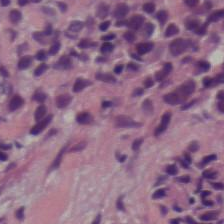
\includegraphics[width=\textwidth]{figures/ejemplos_clase/parches/her2_01plus}
\caption{0/1+}
\end{subfigure}\hfill
\begin{subfigure}[b]{0.3\textwidth}
\centering
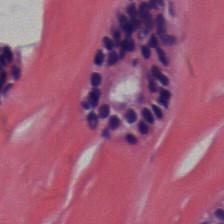
\includegraphics[width=\textwidth]{figures/ejemplos_clase/parches/her2_2plus}
\caption{2+}
\end{subfigure}\hfill
\begin{subfigure}[b]{0.3\textwidth}
\centering
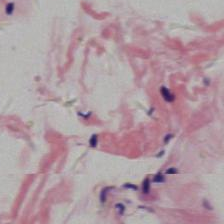
\includegraphics[width=\textwidth]{figures/ejemplos_clase/parches/her2_3plus}
\caption{3+}
\end{subfigure}
\caption{Ejemplos representativos de parches para cada clase de HER2.}
\label{fig:ejemplos_her2}
\end{figure}

\paragraph{Desempeño por modelo y dataset.} En BCNB, la BA osciló entre 0,418 (Phikon-v2) y 0,455 (UNI2), con AUC macro entre 0,602 y 0,632: todos los modelos superan el nivel de referencia de 0,333 correspondiente a tres clases, aunque con una ganancia limitada. En HISTAI-Breast el desempeño desciende a 0,364--0,381, también cercano al nivel de referencia. En HSI-BC, donde solo están presentes dos clases y el nivel de referencia es 0,5, UNI2 (0,438), Virchow2 (0,417) y Phikon-v2 (0,278) quedan por debajo de él, mientras que Prov-GigaPath alcanza 0,562 con IC95\% de [0,359, 0,762]; la amplitud de este intervalo, junto con el tamaño de cohorte de $n=44$, impide establecer una ventaja concluyente (Figura~\ref{fig:ba_her2}).

El análisis por clase muestra una marcada heterogeneidad. En las cohortes grandes, la categoría 2+ es la mejor detectada (sensibilidad de 0,573--0,625 en BCNB y 0,709--0,747 en HISTAI-Breast), en línea con su condición de clase mayoritaria (45,7\% y 63,2\% de los casos, respectivamente), mientras que 0/1+ y 3+ se detectan de forma deficiente (0,140--0,403). En HSI-BC, Virchow2 y Phikon-v2 no identifican ningún caso de 3+ (sensibilidad 0,000), aunque esta observación se basa en un número reducido de pacientes. El AUC es coherente con este patrón: sobre HSI-BC, UNI2 (0,389) y Phikon-v2 (0,184) presentan valores por debajo del azar, lo que, dado el reducido tamaño de la cohorte, indica ausencia de señal aprendida o ruido muestral extremo. Los valores numéricos completos se presentan en las Tablas~\ref{tab:anexo_her2_utilidad}, \ref{tab:anexo_her2_sensibilidad}--\ref{tab:anexo_her2_sensibilidad_hsibc}, \ref{tab:anexo_her2_fairness}--\ref{tab:anexo_her2_fairness_hsibc} y \ref{tab:anexo_her2_crossdataset} del Apéndice~\ref{anexo:resultados_completos}.

\begin{figure}[htbp]
\centering
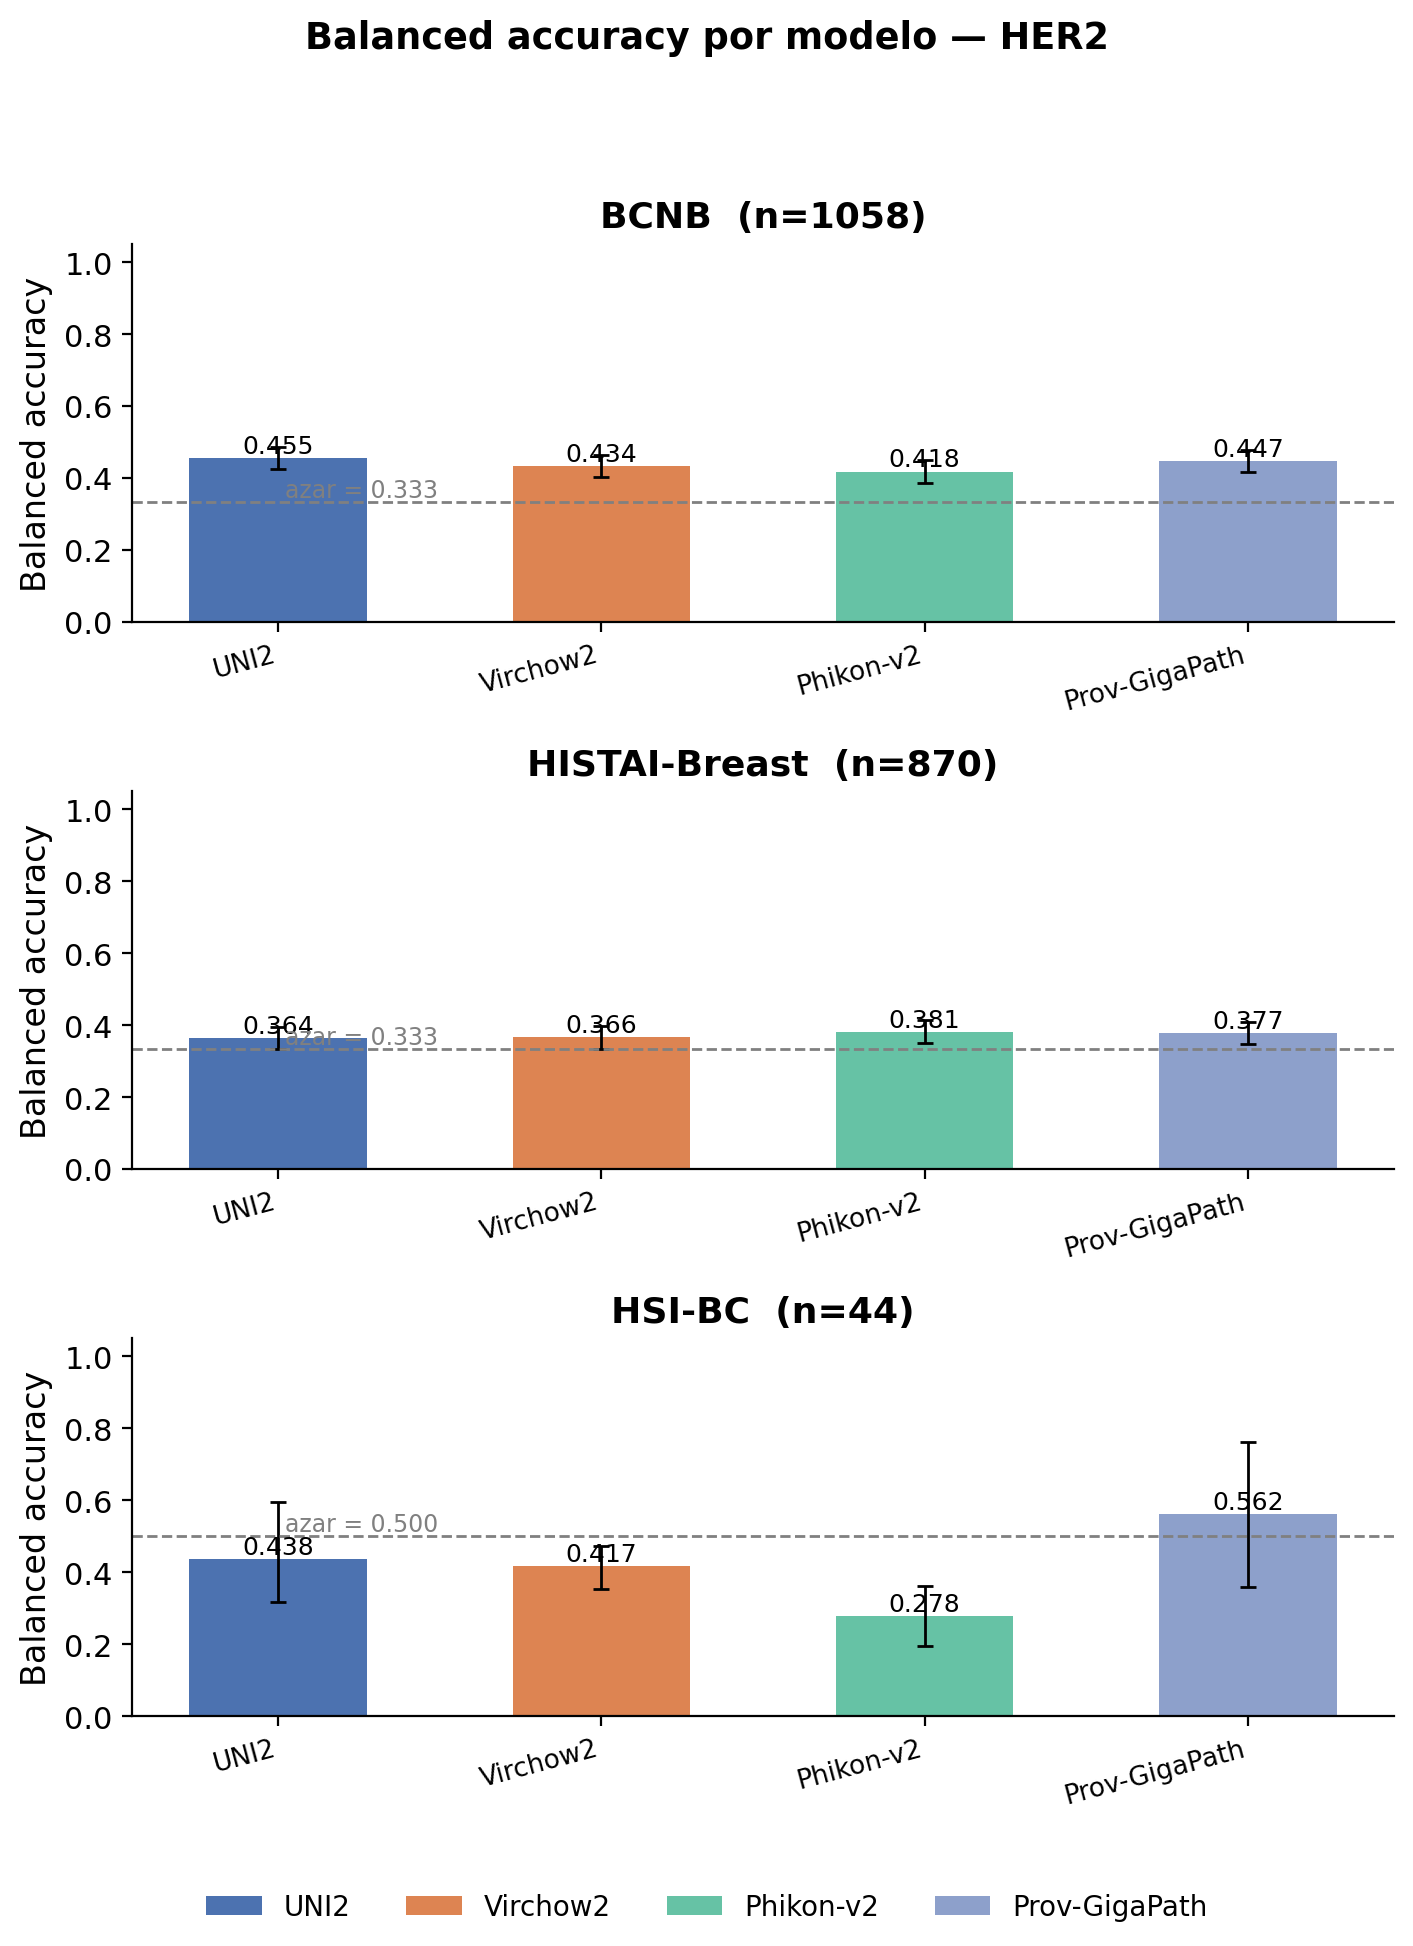
\includegraphics[width=0.75\textwidth]{figures/balanced_accuracy/her2}
\caption{Balanced accuracy por modelo y conjunto de datos en la tarea HER2. Barras de error: IC 95\% bootstrap.}
\label{fig:ba_her2}
\end{figure}

\paragraph{Equidad entre subgrupos.} En BCNB, las brechas de BA por edad variaron entre modelos: UNI2 y Phikon-v2 presentaron las brechas más altas (0,113 y 0,105, respectivamente, con el grupo de $\geq 70$ años como el de mayor desempeño y el de $<50$ años como el de menor), mientras que Virchow2 y Prov-GigaPath presentaron brechas menores (0,032 y 0,019). En HISTAI-Breast, las brechas oscilaron entre 0,022 y 0,065, pero la dirección de la diferencia no fue consistente entre encoders: el grupo de mayor desempeño varía según el modelo evaluado. En HSI-BC, solo los grupos de 50--70 y $\geq 70$ años cumplen el umbral mínimo de inclusión ($n=26$ y $n=14$); las brechas estimadas varían entre 0,003 y 0,123, pero los intervalos de confianza son amplios, por lo que los resultados deben considerarse exploratorios y no permiten inferir de manera robusta la presencia o ausencia de disparidad por edad. No se observó una dirección de favorecimiento consistente entre encoders en las cohortes grandes.

\paragraph{Generalización cross-dataset.} La transferencia BCNB $\rightarrow$ HISTAI-Breast redujo la BA en 0,075--0,108 (16,5--24,1\%), y la transferencia inversa en 0,031--0,055 (8,4--14,4\%). Este patrón es compatible con una mayor proximidad entre ambas cohortes que la observada respecto de HSI-BC; sin embargo, el diseño no permite atribuir esta diferencia exclusivamente a similitudes morfológicas, ya que pueden intervenir factores de adquisición, composición clínica, prevalencia de clases y calidad de las etiquetas. Las transferencias que involucran HSI-BC combinan un cambio de cohorte con un cambio en el número de clases efectivamente evaluadas (la cohorte no contiene la categoría 2+) y, por ello, no son directamente comparables con las transferencias entre BCNB e HISTAI-Breast. Cuando HSI-BC actúa como fuente de entrenamiento, algunos modelos presentan valores OOD superiores a sus valores ID (p.\ ej., $\Delta M = -0{,}249$ para Phikon-v2 al evaluar en BCNB); este resultado no debe interpretarse como generalización superior, sino como una consecuencia posible de la estimación inestable del desempeño ID en una cohorte pequeña y con dos clases.

\paragraph{Síntesis.} En conjunto, T1 muestra una utilidad predictiva limitada bajo el protocolo de extracción de características congeladas y clasificación a nivel de paciente utilizado en este estudio: incluso en las cohortes de mayor tamaño, la BA supera el nivel de referencia por un margen acotado y la sensibilidad se concentra en la categoría 2+. Este comportamiento es compatible con la relación indirecta entre la morfología H\&E y un biomarcador definido mediante inmunohistoquímica, así como con el efecto del desbalance de clases, aunque el diseño no permite separar la contribución de ambos factores. Las diferencias entre cohortes son coherentes con las limitaciones documentadas en el Capítulo~\ref{cap:caracterizacion_datasets}: BCNB presenta el desempeño más alto y estable; HISTAI-Breast alcanza resultados menores en un contexto donde la obtención de biomarcadores desde texto libre puede introducir incertidumbre de etiquetado; y HSI-BC concentra la mayor inestabilidad debido a su tamaño reducido y su limitada representación de clases. Respecto de la equidad, no se observa una dirección de favorecimiento consistente entre modelos y cohortes, por lo que los resultados constituyen una caracterización exploratoria de posibles disparidades, no evidencia definitiva de equidad o inequidad por edad.

\subsection{T2: Subtipo molecular}
\label{sec:resultado_molsub}

\paragraph{Descripción de la tarea y distribución de clases.} T2 clasifica el subtipo molecular del cáncer de mama en cuatro categorías: Luminal A, Luminal B, HER2+ y triple negativo. En BCNB ($n=1.058$) la distribución es relativamente equilibrada (Luminal B 35,2\%, Luminal A 27,2\%, HER2+ 25,8\%, triple negativo 11,8\%); en HISTAI-Breast ($n=842$) domina Luminal B (41,6\%) y triple negativo es minoritaria (8,8\%); en HSI-BC ($n=44$) Luminal B concentra el 63,6\% de los casos y HER2+ cuenta con solo tres casos. La Figura~\ref{fig:ejemplos_molsub} muestra parches ejemplares representativos de cada clase, y la Figura~\ref{fig:anexo_dist_molsub} del Apéndice~\ref{anexo:figuras_distribucion}, la distribución de clases por conjunto de datos.

\begin{figure}[htbp]
\centering
\begin{subfigure}[b]{0.45\textwidth}
\centering
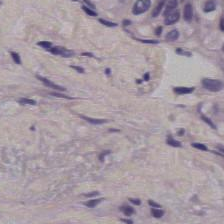
\includegraphics[width=\textwidth]{figures/ejemplos_clase/parches/molsub_her2plus}
\caption{HER2+}
\end{subfigure}\hfill
\begin{subfigure}[b]{0.45\textwidth}
\centering
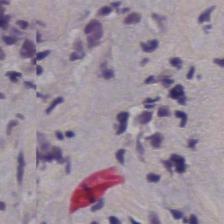
\includegraphics[width=\textwidth]{figures/ejemplos_clase/parches/molsub_luminal_a}
\caption{Luminal A}
\end{subfigure}
\\[2ex]
\begin{subfigure}[b]{0.45\textwidth}
\centering
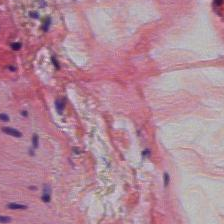
\includegraphics[width=\textwidth]{figures/ejemplos_clase/parches/molsub_luminal_b}
\caption{Luminal B}
\end{subfigure}\hfill
\begin{subfigure}[b]{0.45\textwidth}
\centering
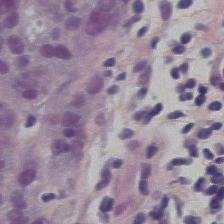
\includegraphics[width=\textwidth]{figures/ejemplos_clase/parches/molsub_triple_neg}
\caption{Triple Negative}
\end{subfigure}
\caption{Ejemplos representativos de parches para cada clase de MolSub.}
\label{fig:ejemplos_molsub}
\end{figure}

\paragraph{Desempeño por modelo y dataset.} BCNB presentó la mayor utilidad: UNI2 alcanzó la mayor BA (0,482; IC95\%: 0,450--0,514), seguido de Prov-GigaPath (0,472), Phikon-v2 (0,434) y Virchow2 (0,427), con AUC macro entre 0,697 y 0,740, superiores a los observados en T1 sobre la misma cohorte. Bajo el protocolo utilizado, este resultado indica una mayor capacidad discriminativa para T2 que para T1; sin embargo, la diferencia también puede estar influida por la definición de las etiquetas, su distribución y su calidad. En HISTAI-Breast, la BA disminuyó a 0,327--0,361. En HSI-BC, donde el nivel de referencia para cuatro clases es 0,25, UNI2 y Prov-GigaPath alcanzaron 0,317 y 0,334, mientras que Virchow2 y Phikon-v2 quedaron por debajo de este valor; dado que la cohorte contiene solo 44 pacientes y presenta categorías con escasa representación, estas diferencias deben interpretarse como estimaciones inestables y no como un ordenamiento concluyente entre modelos (Figura~\ref{fig:ba_molsub}).

El análisis por clase evidenció una heterogeneidad relevante. Luminal B fue la categoría con mayor sensibilidad en BCNB y en HISTAI-Breast (0,492--0,617); HER2+ presentó sensibilidades de 0,262--0,403 en las cohortes grandes; triple negativo alcanzó 0,448--0,568 en BCNB, pero disminuyó a 0,216--0,230 en HISTAI-Breast. En HSI-BC, ningún modelo identificó los tres casos de HER2+, por lo que esa sensibilidad igual a cero debe interpretarse principalmente en función del tamaño extremadamente reducido de la categoría. Los valores numéricos completos se presentan en las Tablas~\ref{tab:anexo_molsub_utilidad}, \ref{tab:anexo_molsub_sensibilidad}--\ref{tab:anexo_molsub_sensibilidad_hsibc}, \ref{tab:anexo_molsub_fairness}--\ref{tab:anexo_molsub_fairness_hsibc} y \ref{tab:anexo_molsub_crossdataset} del Apéndice~\ref{anexo:resultados_completos}.

\begin{figure}[htbp]
\centering
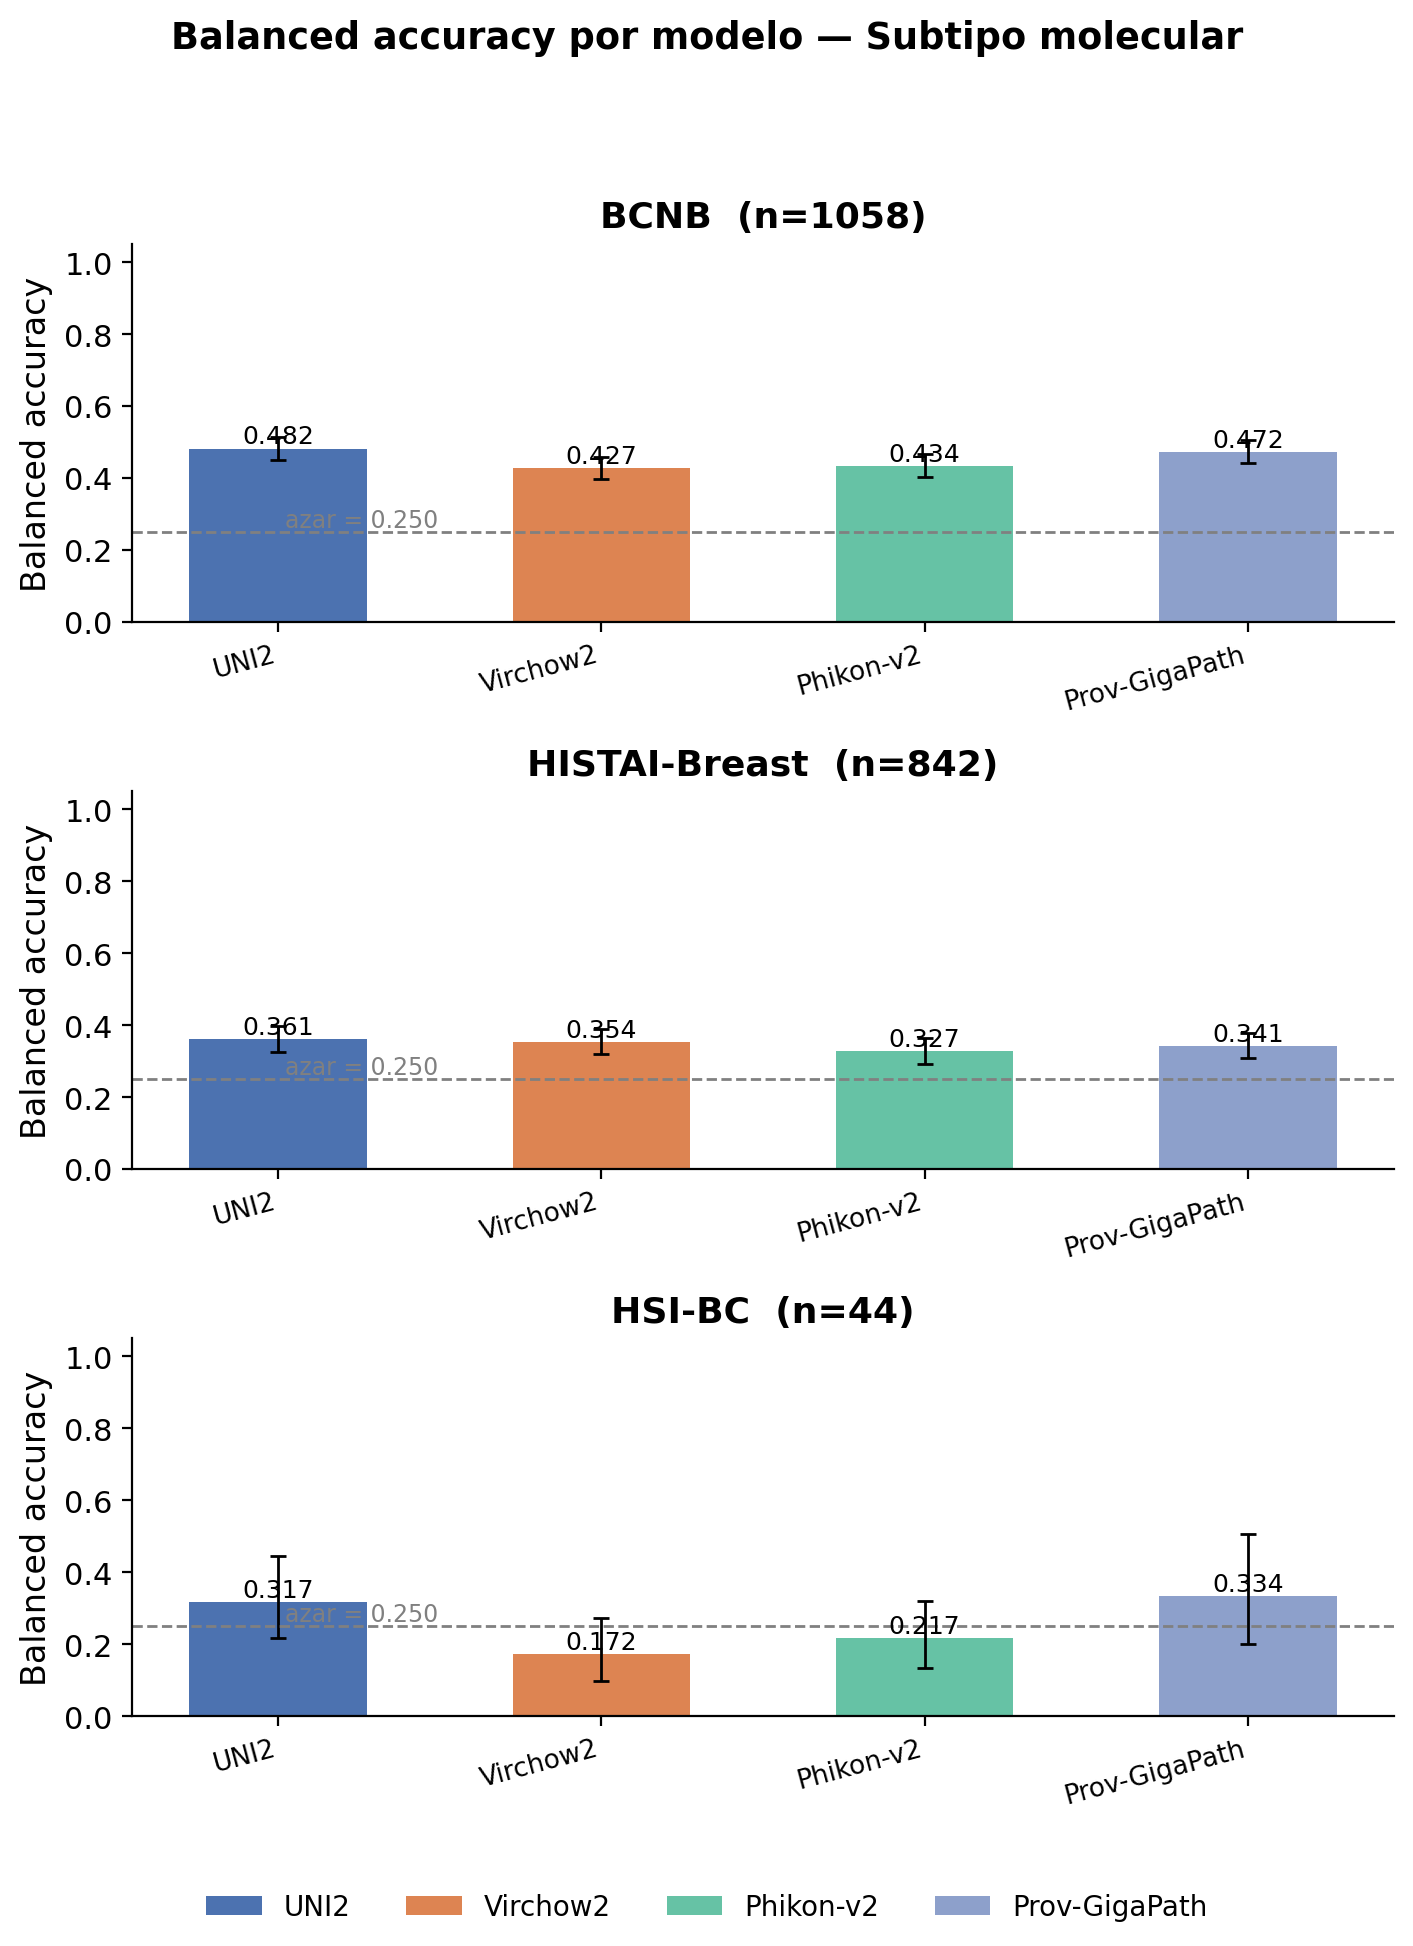
\includegraphics[width=0.72\textwidth]{figures/balanced_accuracy/molsub}
\caption{Balanced accuracy por modelo y conjunto de datos en la tarea MolSub. Barras de error: IC 95\% bootstrap.}
\label{fig:ba_molsub}
\end{figure}

\paragraph{Equidad entre subgrupos.} En BCNB, las brechas de BA por edad variaron entre modelos: Virchow2 y Phikon-v2 presentaron las brechas más bajas (0,010 y 0,023, respectivamente), mientras que UNI2 y Prov-GigaPath alcanzaron 0,078 y 0,041. La dirección de las diferencias no fue uniforme: el grupo de menor edad obtiene el mayor desempeño en UNI2, mientras que en Phikon-v2 el grupo de $\geq 70$ años registra el mayor desempeño; el grupo de $\geq 70$ años registra el menor desempeño en UNI2 y Prov-GigaPath. Por tanto, no se observa un grupo etario favorecido de manera consistente entre los cuatro modelos. En HISTAI-Breast, las brechas variaron entre 0,063 (UNI2) y 0,107 (Virchow2), con grupos de mejor desempeño que cambian según el modelo; estas diferencias deben interpretarse considerando el sesgo de selección hacia pacientes mayores en la cohorte analítica. En HSI-BC, las brechas variaron entre 0,074 y 0,426; la mayor correspondió a Prov-GigaPath, con BA de 0,593 en el grupo de 50--70 años y de 0,190 en el de $\geq 70$, sobre subgrupos de $n=26$ y $n=14$. Además, en cohortes pequeñas y tareas multiclase, la comparación de BA por subgrupo puede estar condicionada por la ausencia o escasa presencia de algunas categorías dentro de cada grupo etario. Por esta razón, las brechas reportadas describen diferencias observadas en esta muestra, pero no deben interpretarse como estimaciones estables de equidad poblacional.

\paragraph{Generalización cross-dataset.} La transferencia desde BCNB hacia HISTAI-Breast redujo la BA en 0,070--0,163, equivalentes a pérdidas relativas de 16,5\% a 34,6\%; la magnitud de la caída varió entre modelos: Virchow2 presentó la menor reducción, mientras que Prov-GigaPath y UNI2 registraron las mayores. Estos resultados indican una pérdida de rendimiento al trasladar el clasificador a una cohorte externa, aunque el diseño no permite separar la contribución de las diferencias de adquisición, composición clínica, prevalencia de subtipos y calidad de las etiquetas. La transferencia hacia HSI-BC presentó resultados más variables: UNI2 y Virchow2 registraron caídas de 0,253 y 0,205, Phikon-v2 de 0,108, y Prov-GigaPath una diferencia reducida de 0,004; este último resultado no debe interpretarse por sí solo como evidencia de robustez superior, ya que HSI-BC es una cohorte pequeña, con distribución de clases distinta y categorías muy escasas. Cuando HSI-BC se utilizó como conjunto de entrenamiento, algunos modelos presentaron valores OOD superiores a su desempeño ID (p.\ ej., $\Delta M = -0{,}096$ para Virchow2 al evaluar en BCNB), patrón compatible con la inestabilidad de la estimación ID en una cohorte pequeña. Los resultados completos se presentan en la Tabla~\ref{tab:anexo_molsub_crossdataset} del Apéndice~\ref{anexo:resultados_completos}.

\paragraph{Síntesis.} T2 presenta una utilidad predictiva mayor que T1 en BCNB, particularmente al considerar el AUC macro: bajo este protocolo, las representaciones fundacionales contienen información más útil para discriminar subtipos moleculares que para clasificar el estado HER2 aislado. Sin embargo, este resultado no permite concluir que la diferencia provenga exclusivamente de una señal morfológica más fuerte, dado que las tareas también difieren en definición de etiquetas, distribución de clases y posibles fuentes de incertidumbre en los metadatos clínicos, en especial la extracción de biomarcadores desde texto libre en HISTAI-Breast. El desempeño disminuye de forma consistente desde BCNB hacia HISTAI-Breast y, con mayor inestabilidad, hacia HSI-BC, un gradiente compatible con las limitaciones documentadas en la caracterización de las cohortes. Respecto de la equidad, no se observa un patrón de favorecimiento consistente entre modelos ni entre cohortes; la brecha elevada de Prov-GigaPath en HSI-BC requiere validación en una cohorte mayor. Los resultados caracterizan posibles disparidades bajo las condiciones evaluadas, pero no permiten afirmar de manera definitiva ni la presencia ni la ausencia de inequidad por edad.

\subsection{T3: Sitio anatómico}
\label{sec:resultado_site}

\paragraph{Descripción de la tarea y distribución de clases.} T3 clasifica el sitio anatómico del tumor colorrectal en nueve categorías: colon derecho, colon transverso, colon izquierdo, sigmoide, rectosigmoide, recto, colon sin especificar, otro y metástasis hepática. En HISTAI-CRC-B1 ($n=878$) predominan sigmoide (24,0\%), recto (18,2\%) y colon derecho (15,4\%); en SurGen ($n=765$) dominan recto (29,8\%) y colon derecho (22,9\%); en HISTAI-CRC-B2 ($n=57$) la clase metástasis hepática está ausente, por lo que la tarea se evalúa con ocho clases, y varias clases cuentan con menos de cinco casos (colon izquierdo 2, rectosigmoide 1, transverso 1). La Figura~\ref{fig:ejemplos_site} muestra parches ejemplares representativos de cada clase, y la Figura~\ref{fig:anexo_dist_site} del Apéndice~\ref{anexo:figuras_distribucion}, la distribución de clases por conjunto de datos.

\begin{figure}[htbp]
\centering
\begin{subfigure}[b]{0.3\textwidth}
\centering
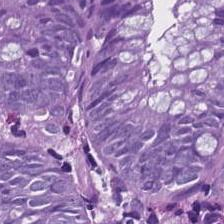
\includegraphics[width=\textwidth]{figures/ejemplos_clase/parches/site_colon_sin_especificar}
\caption{Colon sin especificar}
\end{subfigure}\hfill
\begin{subfigure}[b]{0.3\textwidth}
\centering
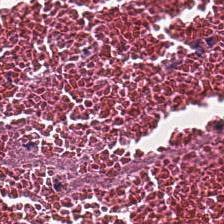
\includegraphics[width=\textwidth]{figures/ejemplos_clase/parches/site_colon_izquierdo}
\caption{Colon izquierdo}
\end{subfigure}\hfill
\begin{subfigure}[b]{0.3\textwidth}
\centering
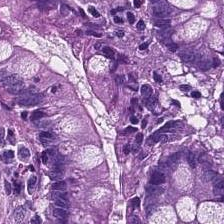
\includegraphics[width=\textwidth]{figures/ejemplos_clase/parches/site_met_higado}
\caption{Metástasis hepática}
\end{subfigure}
\\[2ex]
\begin{subfigure}[b]{0.3\textwidth}
\centering
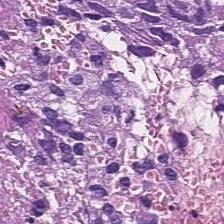
\includegraphics[width=\textwidth]{figures/ejemplos_clase/parches/site_otro}
\caption{Otro}
\end{subfigure}\hfill
\begin{subfigure}[b]{0.3\textwidth}
\centering
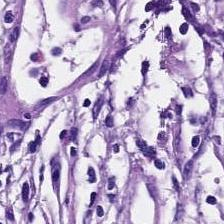
\includegraphics[width=\textwidth]{figures/ejemplos_clase/parches/site_rectosigmoide}
\caption{Rectosigmoide}
\end{subfigure}\hfill
\begin{subfigure}[b]{0.3\textwidth}
\centering
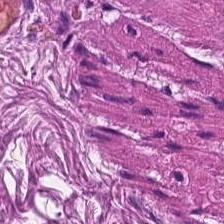
\includegraphics[width=\textwidth]{figures/ejemplos_clase/parches/site_recto}
\caption{Recto}
\end{subfigure}
\\[2ex]
\begin{subfigure}[b]{0.3\textwidth}
\centering
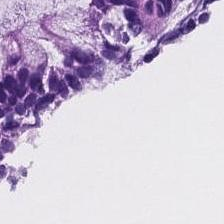
\includegraphics[width=\textwidth]{figures/ejemplos_clase/parches/site_colon_derecho}
\caption{Colon derecho}
\end{subfigure}\hfill
\begin{subfigure}[b]{0.3\textwidth}
\centering
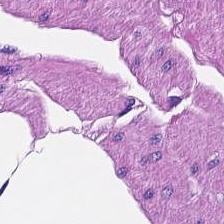
\includegraphics[width=\textwidth]{figures/ejemplos_clase/parches/site_sigmoide}
\caption{Sigmoide}
\end{subfigure}\hfill
\begin{subfigure}[b]{0.3\textwidth}
\centering
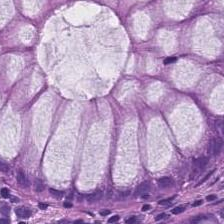
\includegraphics[width=\textwidth]{figures/ejemplos_clase/parches/site_colon_transverso}
\caption{Colon transverso}
\end{subfigure}
\caption{Ejemplos representativos de parches para cada clase de Site.}
\label{fig:ejemplos_site}
\end{figure}

\paragraph{Desempeño por modelo y dataset.} El nivel de referencia de la BA depende del número de clases presentes en cada cohorte: aproximadamente 0,111 para HISTAI-CRC-B1 y SurGen (nueve categorías) y 0,125 para HISTAI-CRC-B2 (ocho categorías). SurGen presentó el mayor desempeño absoluto, con BA de 0,309--0,367 (UNI2 = 0,367; IC95\%: 0,331--0,403); en HISTAI-CRC-B1 los cuatro modelos obtuvieron valores de 0,203--0,210, por sobre el nivel de referencia de una tarea con nueve clases; en HISTAI-CRC-B2, los valores variaron entre 0,094 y 0,138, cercanos al nivel de referencia de ocho clases y acompañados de intervalos de confianza amplios, por lo que esta cohorte no permite una estimación precisa de la utilidad predictiva de los modelos (Figura~\ref{fig:ba_site}).

La sensibilidad por clase fue heterogénea entre cohortes. En SurGen, recto, colon derecho y metástasis hepática alcanzaron máximos de 0,684, 0,480 y 0,886, respectivamente; en HISTAI-CRC-B1, colon derecho y sigmoide alcanzaron sensibilidades de 0,384--0,459, mientras que metástasis hepática no fue identificada por ninguno de los modelos a pesar de estar presente en 18 pacientes. El contraste entre la sensibilidad de metástasis hepática en SurGen y en HISTAI-CRC-B1 es compatible con una influencia de la frecuencia de la clase y de su representatividad dentro de cada cohorte, aunque las cohortes también difieren en adquisición, composición clínica y posibles criterios de anotación. Las categorías rectosigmoide y colon transverso mostraron sensibilidades bajas en las cohortes evaluadas, coherentes con su baja representación. Los valores numéricos completos se presentan en las Tablas~\ref{tab:anexo_site_utilidad}, \ref{tab:anexo_site_sensibilidad}--\ref{tab:anexo_site_sensibilidad_surgen}, \ref{tab:anexo_site_fairness_edad}--\ref{tab:anexo_site_fairness_edad_surgen}, \ref{tab:anexo_site_fairness_sexo}--\ref{tab:anexo_site_fairness_sexo_surgen} y \ref{tab:anexo_site_crossdataset} del Apéndice~\ref{anexo:resultados_completos}.

\begin{figure}[htbp]
\centering
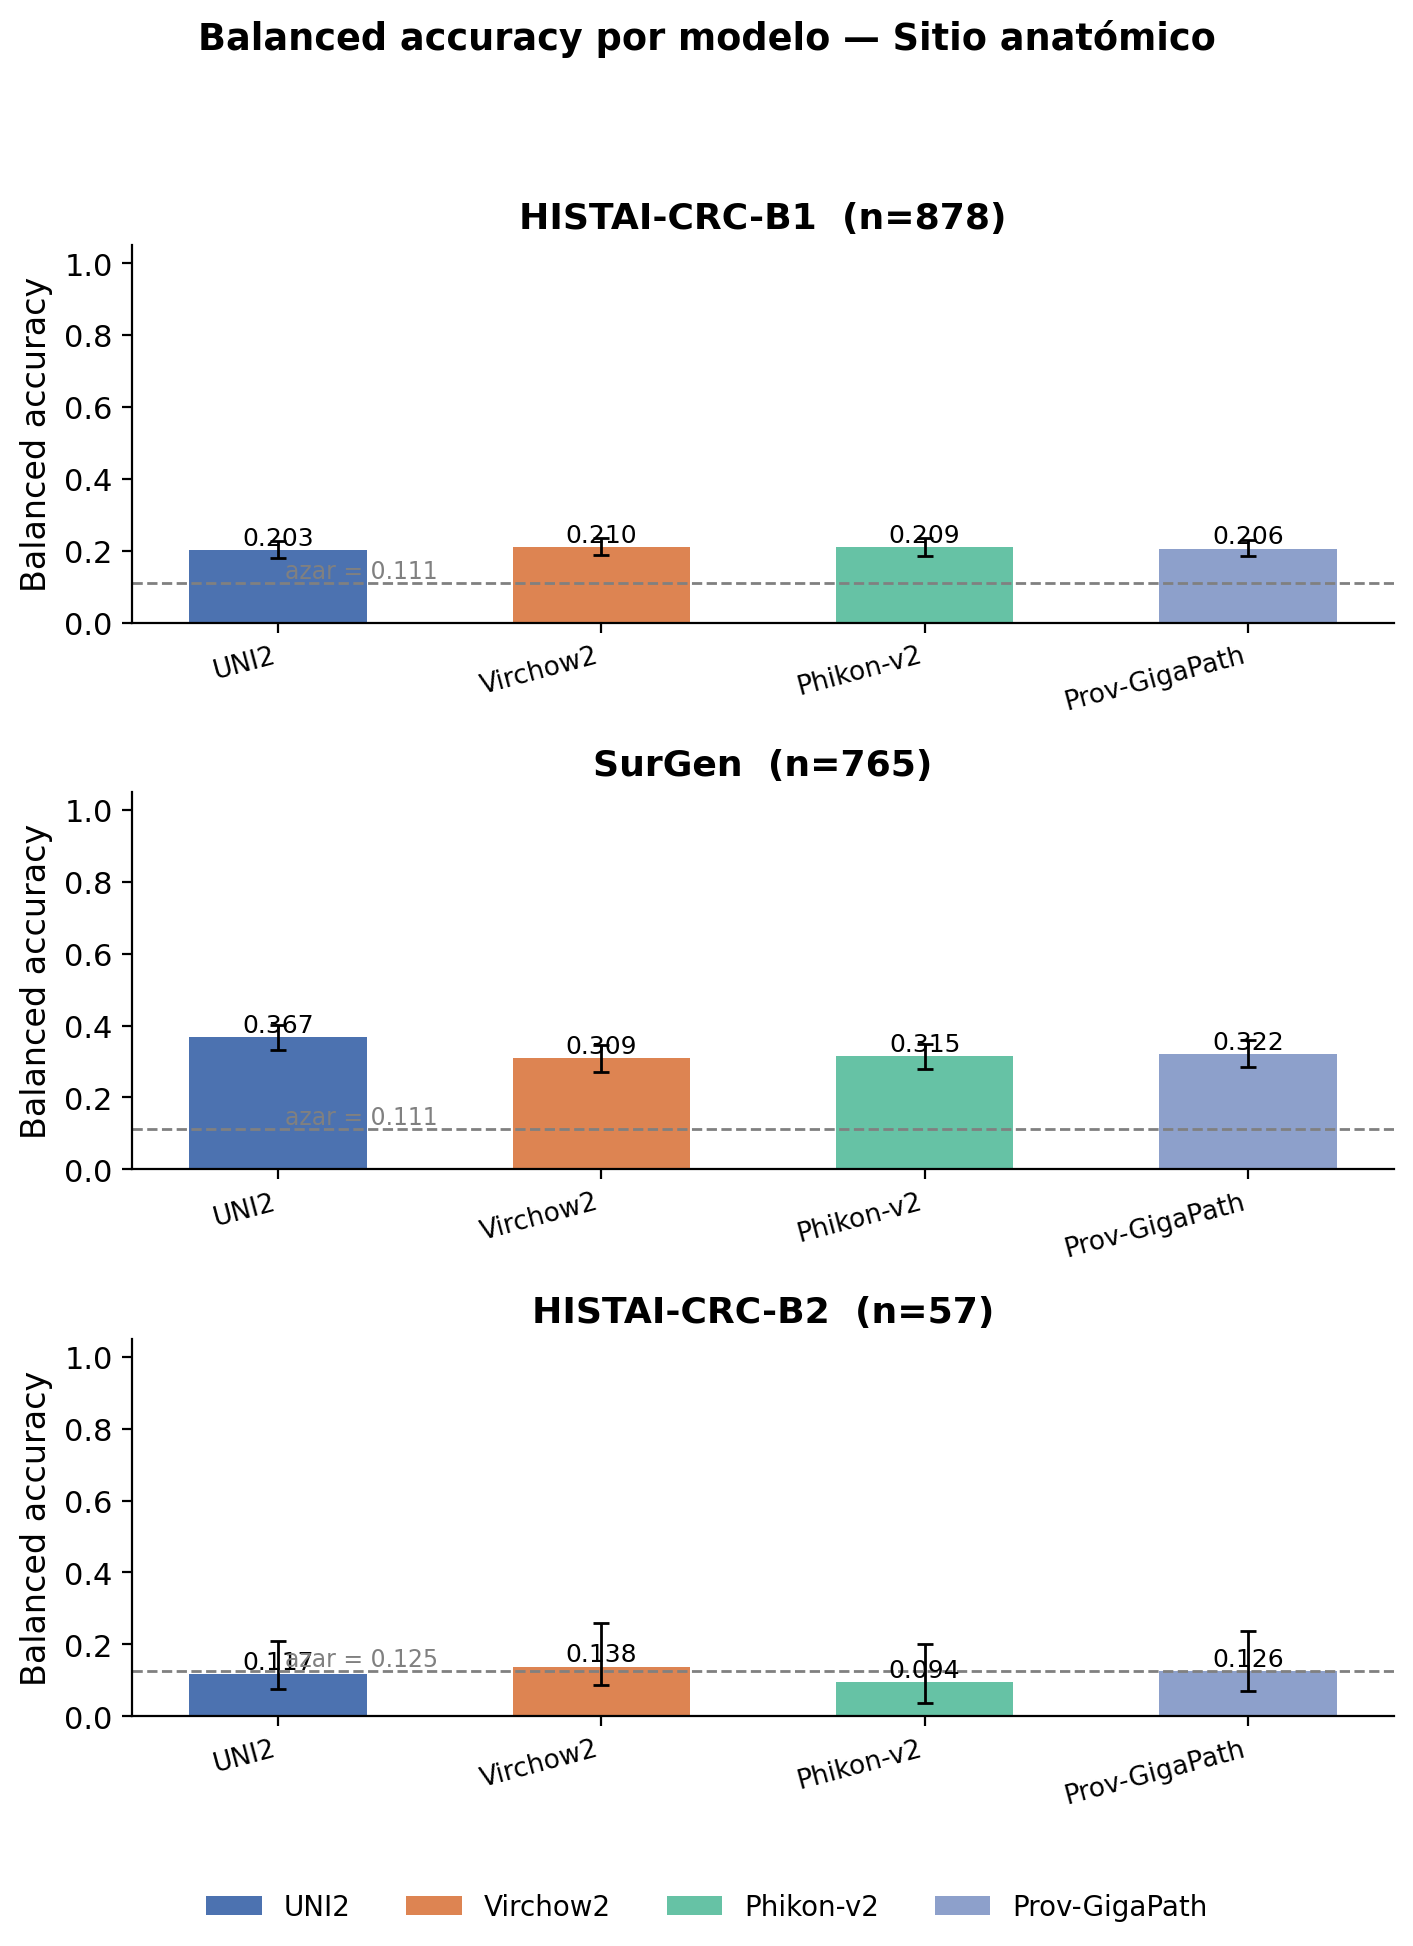
\includegraphics[width=0.72\textwidth]{figures/balanced_accuracy/site}
\caption{Balanced accuracy por modelo y conjunto de datos en la tarea Site. Barras de error: IC 95\% bootstrap.}
\label{fig:ba_site}
\end{figure}

\paragraph{Equidad entre subgrupos.} En las cohortes grandes, las brechas por edad fueron de magnitud reducida a moderada: entre 0,018 y 0,049 en HISTAI-CRC-B1 y entre 0,026 y 0,072 en SurGen. Las brechas por sexo también fueron acotadas en estas cohortes, con valores entre 0,026 y 0,046 en HISTAI-CRC-B1 y entre 0,002 y 0,063 en SurGen. La dirección de las diferencias varió entre modelos, por lo que no se observa un subgrupo de edad o sexo favorecido de manera consistente. En HISTAI-CRC-B2, los análisis por edad incluyeron únicamente los grupos de 50--70 y $\geq 70$ años ($n=25$ y $n=27$, respectivamente): las brechas estimadas variaron entre 0,053 y 0,360, con la mayor correspondiente a Phikon-v2 (IC95\%: [0,015, 0,778]); por sexo ($n=32$ mujeres y $n=25$ hombres), Phikon-v2 presentó una diferencia de 0,201, con BA de 0,201 en mujeres y 0,000 en hombres. Estas estimaciones deben interpretarse de forma exploratoria: el tamaño total de la cohorte es reducido, algunas categorías tienen muy pocos pacientes y la composición de clases puede diferir entre subgrupos, por lo que las diferencias observadas no permiten establecer de manera robusta si existe una disparidad real por edad o sexo.

\paragraph{Generalización cross-dataset.} La generalización entre cohortes colorrectales mostró caídas relevantes. Cuando SurGen actuó como conjunto de entrenamiento, la transferencia hacia HISTAI-CRC-B1 redujo la BA entre 0,166 y 0,238 (51,6--73,4\%), y hacia HISTAI-CRC-B2 entre 0,107 y 0,195, aunque esta última debe interpretarse con especial cautela por el tamaño reducido de la cohorte de destino y la ausencia de una de las categorías anatómicas. En la dirección HISTAI-CRC-B1 hacia SurGen, las caídas se situaron entre 0,081 y 0,106 (38,8--50,3\%). La asimetría entre direcciones muestra que la transferibilidad depende tanto de la cohorte de entrenamiento como de la de evaluación, resultado compatible con diferencias de distribución entre datasets, sin que el diseño permita identificar si estas provienen principalmente de factores técnicos, composición clínica, distribución de sitios anatómicos o procedimientos de anotación. Cuando HISTAI-CRC-B2 se utilizó como fuente de entrenamiento, algunos resultados OOD superaron el desempeño ID; dado que el desempeño ID de esta cohorte es cercano al nivel de referencia y se estima sobre solo 57 pacientes, los deltas negativos deben interpretarse como evidencia de inestabilidad de la estimación ID, no como una demostración de generalización externa. Los resultados completos se presentan en la Tabla~\ref{tab:anexo_site_crossdataset} del Apéndice~\ref{anexo:resultados_completos}.

\paragraph{Síntesis.} T3 es una tarea de alta complejidad: combina un número elevado de categorías anatómicas, distribuciones de clase asimétricas y clases con soporte muy reducido. Por ello, su BA debe interpretarse en relación con el nivel de referencia de una tarea de ocho o nueve clases, y no compararse de manera directa con las tareas binarias o de menor granularidad del capítulo. SurGen alcanza el mejor desempeño absoluto, HISTAI-CRC-B1 obtiene resultados moderados sobre el nivel de referencia, y HISTAI-CRC-B2 no proporciona evidencia suficiente para una evaluación estable de utilidad predictiva, equidad o generalización. La detección desigual de metástasis hepática entre SurGen e HISTAI-CRC-B1 ilustra que el desempeño por clase puede estar condicionado simultáneamente por prevalencia, representatividad de las muestras y diferencias entre cohortes. Respecto de la equidad, las cohortes grandes no muestran un patrón consistente de favorecimiento por edad o sexo; sin embargo, la utilidad predictiva global es limitada en esta tarea, por lo que brechas pequeñas no deben interpretarse por sí solas como evidencia de un desempeño equitativo clínicamente satisfactorio.

\subsection{T4: Lateralidad}
\label{sec:resultado_side}

\paragraph{Descripción de la tarea y distribución de clases.} T4 agrupa la localización del tumor colorrectal en cinco categorías: izquierdo, derecho, recto, rectosigmoide y transverso. En HISTAI-CRC-B1 ($n=615$) predominan izquierdo (39,7\%) y recto (26,0\%); en SurGen ($n=631$) la distribución es más equilibrada (recto 36,1\%, derecho 27,7\%, izquierdo 26,9\%); en HISTAI-CRC-B2 ($n=46$) las clases rectosigmoide y transverso cuentan con un caso cada una. La Figura~\ref{fig:ejemplos_side} muestra parches ejemplares representativos de cada clase, y la Figura~\ref{fig:anexo_dist_side} del Apéndice~\ref{anexo:figuras_distribucion}, la distribución de clases por conjunto de datos.

\begin{figure}[htbp]
\centering
\begin{subfigure}[b]{0.3\textwidth}
\centering
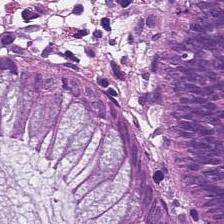
\includegraphics[width=\textwidth]{figures/ejemplos_clase/parches/side_izquierdo}
\caption{Izquierdo}
\end{subfigure}\hfill
\begin{subfigure}[b]{0.3\textwidth}
\centering
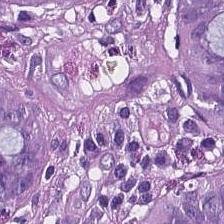
\includegraphics[width=\textwidth]{figures/ejemplos_clase/parches/side_rectosigmoide}
\caption{Rectosigmoide}
\end{subfigure}\hfill
\begin{subfigure}[b]{0.3\textwidth}
\centering
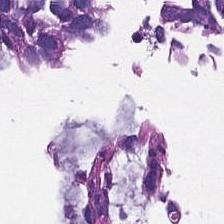
\includegraphics[width=\textwidth]{figures/ejemplos_clase/parches/side_recto}
\caption{Recto}
\end{subfigure}
\\[2ex]
\begin{minipage}{0.62\textwidth}
\centering
\begin{subfigure}[b]{0.48\textwidth}
\centering
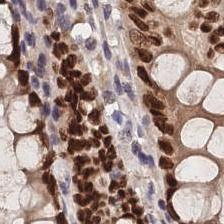
\includegraphics[width=\textwidth]{figures/ejemplos_clase/parches/side_derecho}
\caption{Derecho}
\end{subfigure}\hfill
\begin{subfigure}[b]{0.48\textwidth}
\centering
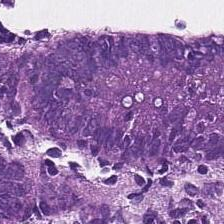
\includegraphics[width=\textwidth]{figures/ejemplos_clase/parches/side_transverso}
\caption{Transverso}
\end{subfigure}
\end{minipage}
\caption{Ejemplos representativos de parches para cada clase de Side.}
\label{fig:ejemplos_side}
\end{figure}

\paragraph{Desempeño por modelo y dataset.} La tarea comprende cinco categorías, por lo que el nivel de referencia uniforme de la BA corresponde a 0,2. En SurGen, UNI2 alcanzó la mayor BA (0,372; IC95\%: 0,329--0,415), seguido de Virchow2 (0,339), Phikon-v2 (0,321) y Prov-GigaPath (0,318); en HISTAI-CRC-B1, los resultados variaron entre 0,293 (Phikon-v2) y 0,331 (Prov-GigaPath). Ambas cohortes superan el nivel de referencia, aunque con una utilidad predictiva todavía moderada (Figura~\ref{fig:ba_side}). En HISTAI-CRC-B2, los cuatro modelos obtuvieron valores entre 0,115 y 0,174, inferiores al nivel de referencia; con solo 46 pacientes y dos categorías con un único caso, la BA y las sensibilidades por clase tienen una elevada variabilidad y no permiten establecer un ordenamiento confiable entre modelos.

El análisis por clase mostró diferencias relevantes entre cohortes: en HISTAI-CRC-B1, la categoría izquierdo presentó sensibilidades entre 0,607 y 0,660 y la categoría derecho entre 0,481 y 0,519; en SurGen, recto fue la categoría mejor detectada (0,675--0,737), seguida de derecho (0,434--0,560). En cambio, transverso y rectosigmoide presentaron sensibilidades bajas en las cohortes evaluadas, coherentes con su representación limitada. Los valores numéricos completos se presentan en las Tablas~\ref{tab:anexo_side_utilidad}, \ref{tab:anexo_side_sensibilidad}--\ref{tab:anexo_side_sensibilidad_surgen}, \ref{tab:anexo_side_fairness_edad}--\ref{tab:anexo_side_fairness_edad_surgen}, \ref{tab:anexo_side_fairness_sexo}--\ref{tab:anexo_side_fairness_sexo_surgen} y \ref{tab:anexo_side_crossdataset} del Apéndice~\ref{anexo:resultados_completos}.

\begin{figure}[htbp]
\centering
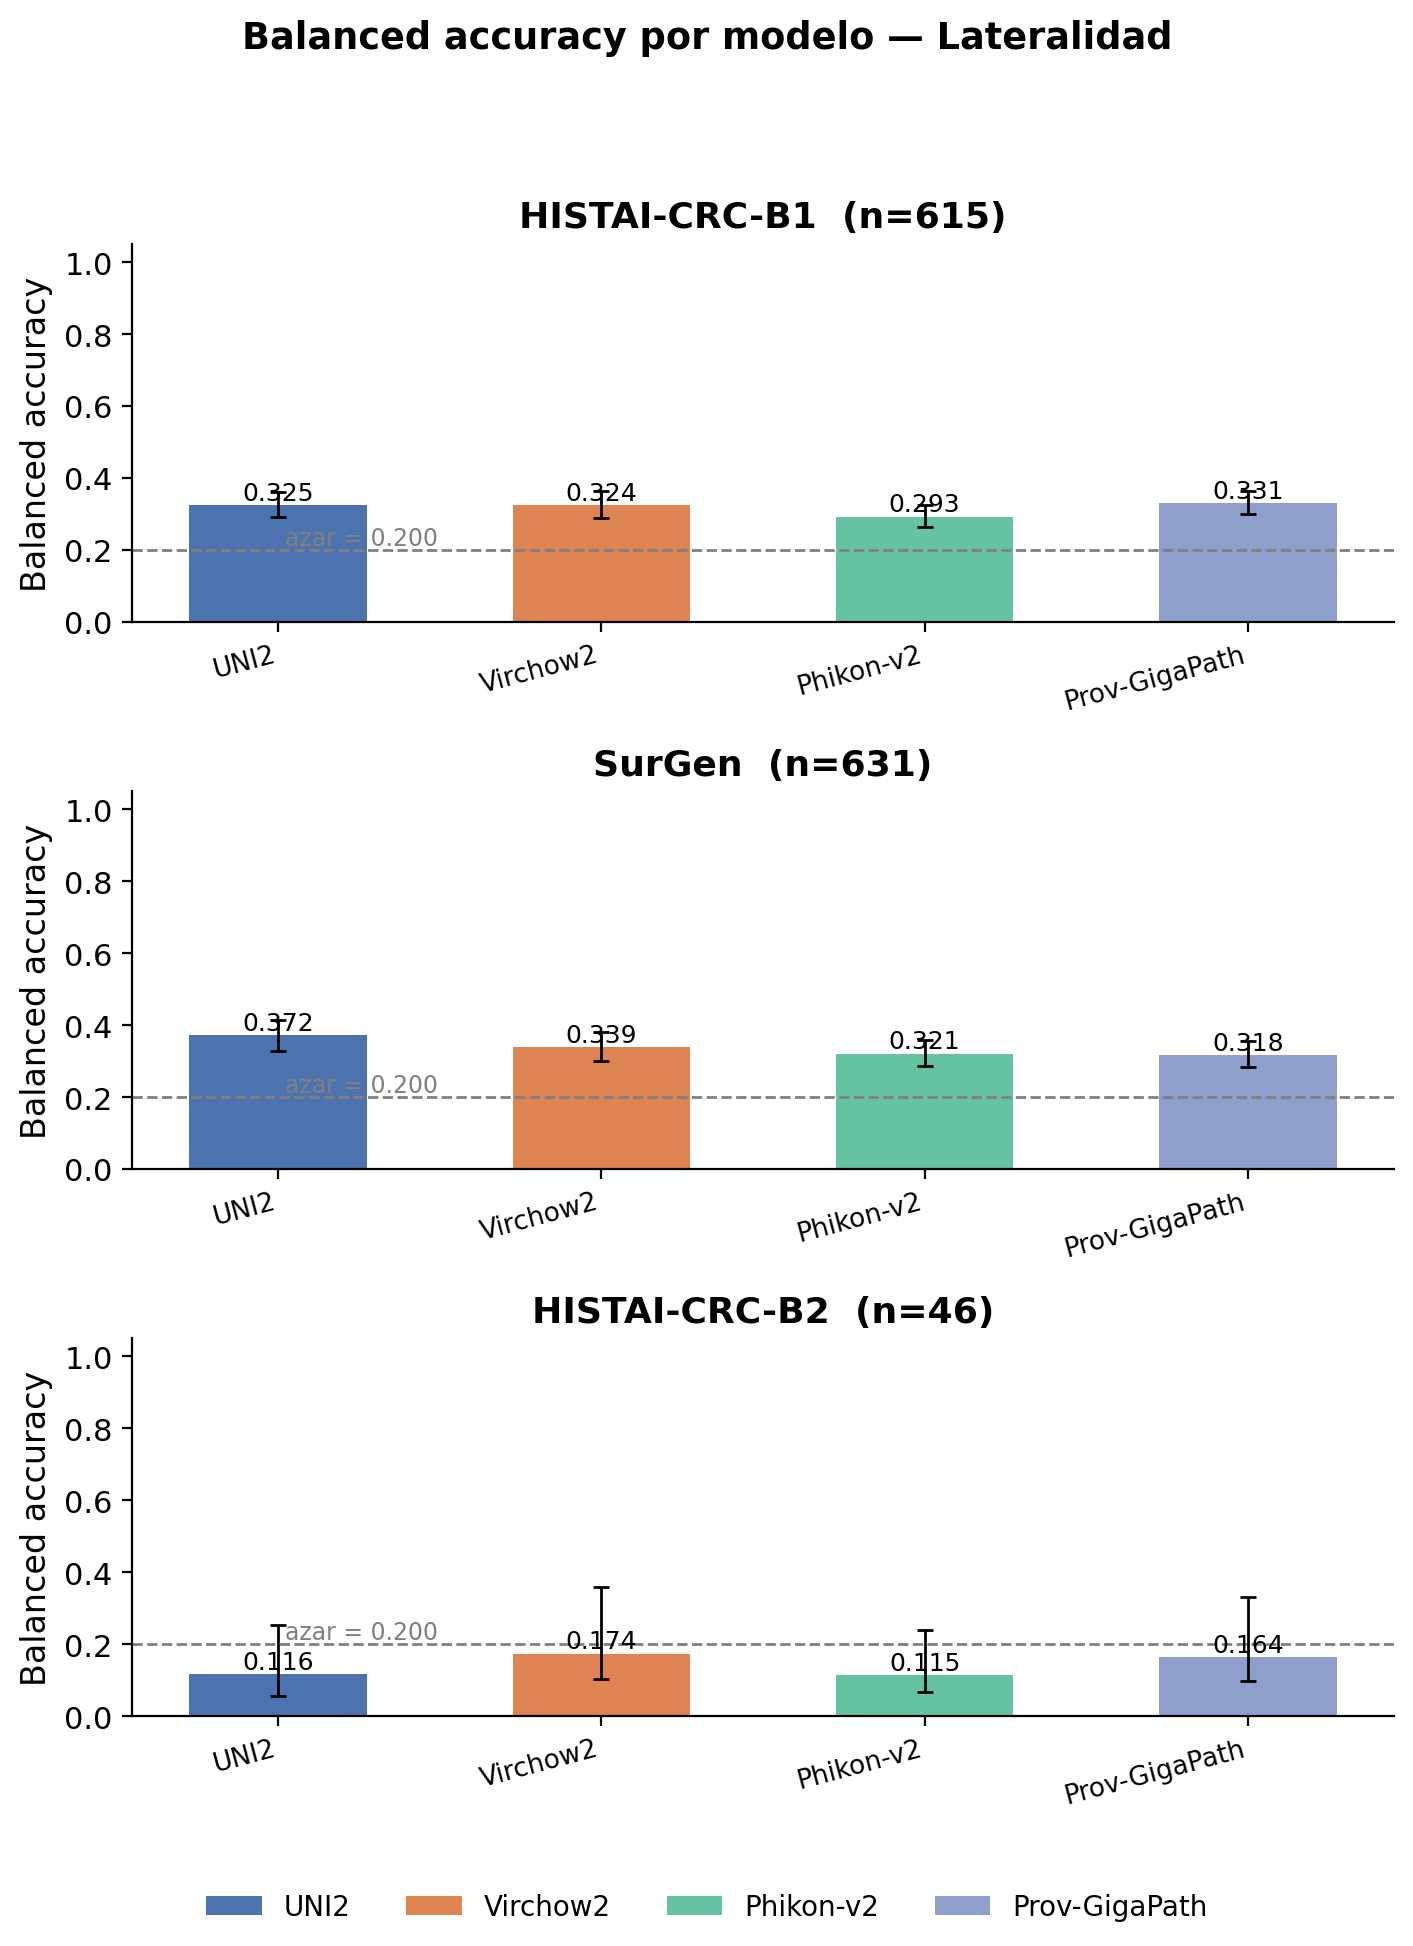
\includegraphics[width=0.72\textwidth]{figures/balanced_accuracy/side}
\caption{Balanced accuracy por modelo y conjunto de datos en la tarea Side. Barras de error: IC 95\% bootstrap.}
\label{fig:ba_side}
\end{figure}

\paragraph{Equidad entre subgrupos.} En HISTAI-CRC-B1, las brechas por edad variaron entre 0,028 y 0,074; en SurGen, entre 0,011 y 0,115 (Phikon-v2 presentó la mayor diferencia por edad y Prov-GigaPath la menor). Las brechas por sexo en las cohortes de mayor tamaño también fueron acotadas, con valores entre 0,032 y 0,061 en HISTAI-CRC-B1 y entre 0,024 y 0,057 en SurGen. La dirección de las diferencias cambia entre modelos, por lo que no se identifica un grupo de edad o sexo favorecido de manera consistente. En HISTAI-CRC-B2, los grupos de edad de 50--70 y $\geq 70$ años incluyen $n=21$ y $n=22$ pacientes: las brechas por edad variaron entre 0,076 y 0,193; por sexo, la cohorte incluye $n=26$ mujeres y $n=20$ hombres, con brechas entre 0,136 y 0,306 (Prov-GigaPath presentó la diferencia más alta, con BA de 0,373 en mujeres y de 0,067 en hombres). Las diferencias observadas en HISTAI-CRC-B2 deben interpretarse de manera exploratoria: en este contexto, una BA cercana a cero en un grupo no permite por sí sola concluir que exista sesgo por sexo o edad; se requiere una cohorte externa de mayor tamaño y con soporte suficiente por categoría para evaluar esa hipótesis.

\paragraph{Generalización cross-dataset.} La transferencia entre las cohortes colorrectales mostró caídas relevantes de rendimiento. Cuando SurGen actuó como conjunto de entrenamiento, la transferencia hacia HISTAI-CRC-B1 redujo la BA entre 0,085 y 0,166 (26,8--46,0\%); en la dirección inversa, desde HISTAI-CRC-B1 hacia SurGen, las caídas variaron entre 0,080 y 0,115 (24,6--39,1\%). La transferencia hacia HISTAI-CRC-B2 presentó mayor incertidumbre: UNI2 disminuyó 0,145 y Virchow2 0,205, mientras que Phikon-v2 y Prov-GigaPath presentaron diferencias pequeñas o negativas; dado que HISTAI-CRC-B2 contiene solo 46 pacientes y presenta categorías con soporte mínimo, estas diferencias no permiten comparar de forma confiable la robustez de los modelos frente a cambios de cohorte. Cuando HISTAI-CRC-B2 se utilizó como fuente de entrenamiento, se observaron nuevamente deltas negativos hacia HISTAI-CRC-B1, patrón compatible con una estimación ID inestable en una cohorte pequeña y con desempeño limitado. Los resultados completos se presentan en la Tabla~\ref{tab:anexo_side_crossdataset} del Apéndice~\ref{anexo:resultados_completos}.

\paragraph{Síntesis.} T4 presentó una utilidad predictiva mayor que T3 en las cohortes colorrectales de mayor tamaño, resultado compatible con la menor granularidad de la etiqueta (cinco categorías frente a nueve), aunque ambas tareas no contienen exactamente los mismos pacientes ni la misma distribución de clases. Los resultados por clase muestran que las categorías más representadas, izquierdo, derecho y recto, concentran las sensibilidades más altas, mientras que transverso y rectosigmoide mantienen sensibilidades bajas, patrón compatible con una influencia conjunta de la prevalencia de clases, la heterogeneidad morfológica y la definición de las categorías anatómicas. Respecto de la equidad, HISTAI-CRC-B1 y SurGen no muestran un patrón consistente de favorecimiento por edad o sexo, pero las brechas deben interpretarse junto con la utilidad predictiva global, que sigue siendo moderada; en HISTAI-CRC-B2, las diferencias por edad y sexo son exploratorias y no permiten confirmar ni descartar una disparidad real.

\subsection{T5: Órgano y separabilidad entre cohortes}
\label{sec:resultado_organ}
\label{sec:verificacion_center_effect}

\paragraph{Descripción de la tarea.} T5 clasifica el órgano de origen (mama vs.\ colorrectal) en los 3.675 pacientes integrados (para HSI-BC se usa su cohorte curada completa, $n=47$, pues la etiqueta de órgano está disponible en todos sus casos), con una distribución de 53,7\% para mama y 46,3\% para colorrectal. La tarea debe interpretarse como un experimento auxiliar de separabilidad entre cohortes: ninguna cohorte incluida contiene muestras de ambos órganos, por lo que la etiqueta de órgano está asociada al origen de la cohorte y el clasificador puede utilizar tanto diferencias entre tejidos como señales técnicas o institucionales asociadas al dataset, tales como tinción, escáner, preparación de la muestra o composición clínica.

\paragraph{Desempeño por modelo y dataset.} Los cuatro modelos resolvieron la tarea con desempeño casi perfecto: BA entre 0,996 (Prov-GigaPath) y 1,000 (Virchow2), AUC = 1,000 para los cuatro encoders, sensibilidad de 1,000 para mama en todos los casos y de 0,992--1,000 para colorrectal. Este resultado no debe interpretarse como una validación aislada de clasificación de órgano: demuestra la separabilidad de las cohortes integradas, no una capacidad de clasificación de órgano independiente de los factores de adquisición, institución, composición clínica, anotación y curación, que varían simultáneamente con el órgano. Las brechas por edad (0,000--0,010) están dominadas por un efecto de techo: cuando el desempeño es prácticamente perfecto para todos los grupos, la brecha de rendimiento queda limitada y aporta poca información sobre la capacidad del modelo para mantener un desempeño equitativo en una tarea clínicamente más exigente. La equidad por sexo no se evaluó debido a la cobertura incompleta de esta variable en la cohorte integrada. Los valores numéricos completos se presentan en las Tablas~\ref{tab:anexo_organ_utilidad}, \ref{tab:anexo_organ_sensibilidad} y \ref{tab:anexo_organ_fairness} del Apéndice~\ref{anexo:resultados_completos}.

\paragraph{Verificación experimental del \textit{center effect}.} Para evaluar directamente la señal de origen, se entrenaron clasificadores de dataset sobre los \textit{embeddings}, reutilizando la configuración del protocolo: MLP con 256 unidades ocultas y activación ReLU, $\alpha = 10^{-4}$, \texttt{max\_iter = 500}, sobremuestreo de las clases minoritarias y validación cruzada de cinco pliegues mediante \texttt{StratifiedGroupKFold}, agrupada por paciente y con \texttt{seed = 42}. El Experimento A evalúa la separabilidad entre datasets dentro de cada dominio clínico mediante clasificación de tres cohortes (nivel de referencia 1/3); el Experimento B compara pares de cohortes colorrectales (nivel de referencia 0,5). En el dominio de mama, BCNB, HISTAI-Breast y HSI-BC presentaron una separabilidad prácticamente perfecta dentro de la cohorte común de 1.944 pacientes utilizada en este experimento: los cuatro modelos alcanzaron BA y AUC de 1,000 para clasificar el dataset de origen. Este resultado muestra que los \textit{embeddings} contienen una firma de cohorte muy marcada; sin embargo, las tres cohortes difieren simultáneamente en institución, condiciones de adquisición, composición de pacientes, disponibilidad de metadatos y procesos de curación, por lo que esta comparación no permite atribuir la separación a un factor técnico o biológico específico.

El dominio colorrectal permite un contraste más informativo. HISTAI-CRC-B1 e HISTAI-CRC-B2 comparten el escáner Leica Aperio GT450 AT2, pero su origen sigue siendo altamente recuperable: la clasificación conjunta de SurGen, HISTAI-CRC-B1 e HISTAI-CRC-B2 alcanzó BA de 0,856--0,928 y AUC de 0,991--0,998; incluso HISTAI-CRC-B1 frente a HISTAI-CRC-B2 alcanzó BA de 0,821--0,864 y AUC de 0,970--0,986, mientras que los pares que incluyen SurGen (escáner diferente) alcanzaron BA y AUC de 1,000 (Tabla~\ref{tab:center_effect}). Esto muestra que existen diferencias entre cohortes que permanecen disponibles en las representaciones incluso cuando el escáner es compartido, posiblemente asociadas a tinción, preparación y manejo del tejido, distribución clínica, anotación, calidad de las imágenes u otros factores no observados; a la vez, la diferencia entre la separabilidad de B1 frente a B2 y la separabilidad perfecta de los pares que incluyen SurGen no permite cuantificar una contribución causal específica del escáner.

\begin{table}[htbp]
\centering
\caption{Resumen de la separabilidad entre cohortes mediante clasificación de origen de dataset. Los rangos de \textit{balanced accuracy} corresponden a los cuatro modelos fundacionales evaluados. El detalle completo se presenta en las Tablas~\ref{tab:anexo_center_effect_a} y \ref{tab:anexo_center_effect_b} del Apéndice~\ref{anexo:resultados_completos}.}
\label{tab:center_effect}
\small
\begin{tabular}{p{3.0cm} p{5.6cm} c c}
\toprule
\textbf{Dominio} & \textbf{Comparación} &
\textbf{$n_{\text{eval}}$} & \textbf{BA} \\
\midrule
Mama &
BCNB, HISTAI-Breast y HSI-BC &
1944 &
1.000 \\

Colorrectal &
SurGen, HISTAI-CRC-B1 e HISTAI-CRC-B2 &
1700 &
0.856 a 0.928 \\

Colorrectal &
HISTAI-CRC-B1 frente a HISTAI-CRC-B2, escáner compartido &
935 &
0.821 a 0.864 \\

Colorrectal &
SurGen frente a HISTAI-CRC-B1, escáner diferente &
1643 &
1.000 \\

Colorrectal &
SurGen frente a HISTAI-CRC-B2, escáner diferente &
822 &
1.000 \\
\bottomrule
\end{tabular}

\medskip
\footnotesize
\parbox{0.95\textwidth}{\textit{Nota:} La comparación de mama utiliza la cohorte común de 1944 pacientes disponible para los cuatro encoders, correspondiente a la cohorte analítica de T2-MOLSUB. Por ello, su tamaño difiere del reportado en T1-HER2.}
\end{table}

\paragraph{Síntesis.} Estos experimentos demuestran que el origen de la cohorte es altamente recuperable desde los \textit{embeddings} evaluados, hallazgo consistente con las caídas OOD observadas en T1--T4 y que refuerza la necesidad de interpretar tales caídas como el resultado potencial de múltiples fuentes de cambio de distribución. No permiten asignar causalmente esa separabilidad al escáner ni a un único factor, porque adquisición, institución, composición clínica, anotación y curación varían simultáneamente; el diseño actual no permite determinar qué proporción corresponde a diferencias morfológicas reales, factores técnicos de adquisición o características institucionales y clínicas de las cohortes. El detalle completo de las métricas e intervalos de confianza se presenta en las Tablas~\ref{tab:anexo_center_effect_a} y \ref{tab:anexo_center_effect_b} del Apéndice~\ref{anexo:resultados_completos}.

\section{Síntesis del capítulo}
\label{sec:sintesis_cap6}

La utilidad predictiva dependió principalmente de la tarea y de la cohorte. T2-MOLSUB superó a T1-HER2 en BCNB; en colorrectal, T4-SIDE obtuvo mayor utilidad que T3-SITE, coherente con su menor granularidad. T5-ORGAN fue casi perfecto, pero su interpretación está limitada por la confusión estructural entre órgano y origen de cohorte. La Tabla~\ref{tab:sintesis_utilidad_equidad} resume cualitativamente la utilidad predictiva, la estabilidad de las estimaciones de equidad y la generalización entre cohortes; los colores representan la interpretabilidad de los resultados bajo las condiciones de evaluación y no una clasificación definitiva de equidad, inequidad o sesgo.

\begin{table}[htbp]
\centering
\caption{Síntesis cualitativa de utilidad predictiva, equidad y generalización por tarea y cohorte. Los colores representan la estabilidad e interpretabilidad de los resultados, no una clasificación definitiva de sesgo o equidad.}
\label{tab:sintesis_utilidad_equidad}
\small
\resizebox{\textwidth}{!}{%
\begin{tabular}{l l p{3.2cm} p{3.6cm} p{3.4cm}}
\toprule
\textbf{Tarea} &
\textbf{Cohorte} &
\textbf{Utilidad predictiva} &
\textbf{Equidad por subgrupos} &
\textbf{Generalización} \\
\midrule

T1-HER2 &
BCNB &
\cellcolor{yellow!25}Limitada &
\cellcolor{yellow!25}Brechas variables por edad &
\cellcolor{yellow!25}Caída moderada hacia HISTAI-Breast \\

T1-HER2 &
HISTAI-Breast &
\cellcolor{yellow!25}Limitada &
\cellcolor{green!20}Sin patrón etario consistente &
\cellcolor{yellow!25}Caída moderada hacia BCNB \\

T1-HER2 &
HSI-BC &
\cellcolor{red!25}Exploratoria, $n=44$ &
\cellcolor{red!25}No concluyente &
\cellcolor{red!25}No interpretable de forma estable \\
\midrule

T2-MOLSUB &
BCNB &
\cellcolor{green!20}Mayor utilidad en mama &
\cellcolor{yellow!25}Brechas variables por edad &
\cellcolor{yellow!25}Caída hacia cohortes externas \\

T2-MOLSUB &
HISTAI-Breast &
\cellcolor{yellow!25}Moderada &
\cellcolor{yellow!25}Brechas variables por edad &
\cellcolor{yellow!25}Caída desde BCNB \\

T2-MOLSUB &
HSI-BC &
\cellcolor{red!25}Exploratoria, $n=44$ &
\cellcolor{red!25}No concluyente &
\cellcolor{red!25}No interpretable de forma estable \\
\midrule

T3-SITE &
HISTAI-CRC-B1 &
\cellcolor{yellow!25}Moderada para nueve clases &
\cellcolor{green!20}Sin patrón consistente &
\cellcolor{yellow!25}Caída relevante hacia SurGen \\

T3-SITE &
SurGen &
\cellcolor{green!20}Mayor utilidad de T3 &
\cellcolor{green!20}Sin patrón consistente &
\cellcolor{yellow!25}Caída relevante hacia otras cohortes \\

T3-SITE &
HISTAI-CRC-B2 &
\cellcolor{red!25}Exploratoria, $n=57$ &
\cellcolor{red!25}No concluyente &
\cellcolor{red!25}No interpretable de forma estable \\
\midrule

T4-SIDE &
HISTAI-CRC-B1 &
\cellcolor{yellow!25}Moderada &
\cellcolor{green!20}Sin patrón consistente &
\cellcolor{yellow!25}Caída hacia SurGen \\

T4-SIDE &
SurGen &
\cellcolor{green!20}Mayor utilidad de T4 &
\cellcolor{yellow!25}Brechas variables por edad &
\cellcolor{yellow!25}Caída hacia HISTAI-CRC-B1 \\

T4-SIDE &
HISTAI-CRC-B2 &
\cellcolor{red!25}Exploratoria, $n=46$ &
\cellcolor{red!25}No concluyente &
\cellcolor{red!25}No interpretable de forma estable \\
\midrule

T5-ORGAN &
Cohorte combinada &
\cellcolor{blue!20}Casi perfecta, pero confundida &
\cellcolor{blue!20}Efecto de techo &
\cellcolor{blue!20}No aplica \\
\bottomrule
\end{tabular}%
}

\medskip
\footnotesize
\parbox{0.97\textwidth}{\textit{Nota:} Verde indica resultados relativamente estables y sin un patrón demográfico consistente entre modelos. Amarillo indica resultados interpretables con limitaciones de utilidad, variabilidad entre modelos o caída de generalización. Rojo indica resultados exploratorios, condicionados por tamaño muestral reducido o soporte insuficiente de clases y subgrupos. Azul indica una dimensión no evaluable, no aplicable o dominada por confusión estructural. Los colores no constituyen una clasificación definitiva de equidad, inequidad o sesgo.}
\end{table}

No se identificó un patrón de favorecimiento por edad o sexo que fuese consistente entre encoders y cohortes grandes. Las brechas pequeñas no prueban por sí mismas equidad clínicamente satisfactoria cuando la utilidad global es limitada; las estimaciones de HSI-BC e HISTAI-CRC-B2 son exploratorias por tamaño y soporte de clases.

Las diferencias entre cohortes fueron más consistentes que las diferencias entre modelos fundacionales: ningún encoder dominó de manera transversal en todas las tareas y cohortes. BCNB, SurGen e HISTAI-CRC-B1 presentaron resultados más estables, mientras que HSI-BC e HISTAI-CRC-B2 concentraron la mayor incertidumbre debido a su tamaño reducido, la representación limitada de algunas clases y la menor estabilidad de las estimaciones; HISTAI-Breast presentó resultados intermedios, en un contexto donde la disponibilidad y trazabilidad de biomarcadores constituye una fuente adicional de incertidumbre.

La transferencia entre cohortes produjo caídas relevantes y el origen de dataset fue altamente separable desde los \textit{embeddings}. En consecuencia, la evaluación de modelos fundacionales en patología debe interpretar conjuntamente la tarea clínica, la calidad y trazabilidad de las cohortes, la estabilidad de las métricas por subgrupo y el cambio de distribución entre centros.